% \documentclass[bachelor,nocolorlinks, printoneside]{seuthesis} % 本科
\documentclass[master]{seuthesis} % 硕士
% \documentclass[doctor]{seuthesis} % 博士
% \documentclass[engineering]{seuthesis} % 工程硕士
\usepackage{CJK,CJKnumb}
\usepackage{amsmath}
\usepackage{amsfonts} 
\usepackage{bm} 
\usepackage{algorithm}
\usepackage{algorithmicx}
\usepackage{algpseudocode}
\usepackage{subfigure}

\floatname{algorithm}{算法}
\renewcommand{\algorithmicrequire}{\textbf{输入:}}
\renewcommand{\algorithmicensure}{\textbf{输出:}}
 % 这里是导言区

\begin{document}
\categorynumber{000} % 分类采用《中国图书资料分类法》
\UDC{000}            %《国际十进分类法UDC》的类号
\secretlevel{公开}    %学位论文密级分为"公开"、"内部"、"秘密"和"机密"四种
\studentid{09013000}   %学号要完整,前面的零不能省略。

\title{一种TDD/FDD下低时延宽带无线信道密钥生成系统研究}{}{Deep learning in greek alphabet}{subtitle}
\author{袁瑞}{Rui Yuan}
% \advisor{彭林宁}{副研究员}{Linning Peng}{Associate Prof.}  % 没有
\coadvisor{彭林宁}{副教授}{Linning Peng}{Associate Prof.}

% \degree{工学硕士} % 详细学位名称
\major[12em]{网络空间安全}
\defenddate{答辩日期}
\authorizedate{学位授予日期}
\department{网络空间安全}{department name}
\duration{2017年9月—2020年6月}
\address{东南大学}
% \thanks{本论文获国家XXX计划项目(2012AA00A00)和国家杰出青年科学基金项目(01234567)资助。}
\maketitle

\begin{abstract}{希腊字母,腓尼基字母,语言,深度学习}
希腊字母源自腓尼基字母。腓尼基字母只有辅音,从右向左写。希腊语的元音发达,希腊人增添了元音字母。因为希腊人的书写工具是蜡板,有时前一行从右向左写完后顺势就从左向右写,变成所谓“耕地”式书写,后来逐渐演变成全部从左向右写。字母的方向也颠倒了。罗马人引进希腊字母,略微改变变为拉丁字母,在世界广为流行。希腊字母广泛应用到学术领域,如数学等。

希腊字母是希腊语所使用的字母,是世界上最早的有元音的字母,也广泛使用于数学、物理、生物、天文等学科。俄语等使用的西里尔字母也是由希腊字母演变而成。希腊字母进入了许多语言的词汇中,英语单字“alphabet”(字母表),源自拉丁语“alphabetum”,源自希腊语“αλφαβητον”,即为前两个希腊字母α(“Alpha”)及β(“Beta”)所合成,三角洲(“Delta”)这个词就来自希腊字母Δ,因为Δ是三角形。
\end{abstract}

\begin{englishabstract}{Greek Alphabet, Phoenician Alphabet, Language, Deep Learning}
The Greek alphabet has been used to write the Greek language since the late 9th century BC or early 8th century BC It was derived from the earlier Phoenician alphabet, and was the first alphabetic script to have distinct letters for vowels as well as consonants. It is the ancestor of the Latin and Cyrillic scripts.Apart from its use in writing the Greek language, in both its ancient and its modern forms, the Greek alphabet today also serves as a source of technical symbols and labels in many domains of mathematics, science and other fields.

In its classical and modern forms, the alphabet has 24 letters, ordered from alpha to omega. Like Latin and Cyrillic, Greek originally had only a single form of each letter; it developed the letter case distinction between upper-case and lower-case forms in parallel with Latin during the modern era.
\end{englishabstract}

\tableofcontents

% \begin{terminology}
% \begin{table}[h]
% \renewcommand\arraystretch{1.5}
% %\Large
% \begin{tabular}{>{\LARGE}m{0.2\textwidth} <{\centering}m{0.7\textwidth}}
% a & 如同汉字起源于象形,拉丁字母表中的每个字母一开始都是描摹某种动物或物体形状的图画\\

% b&和A一样,字母B也可以追溯到古代腓尼基。在腓尼基字母表中B叫beth,代表房屋,在希伯来语中B也叫beth,也含房屋之意。\\

% c& 字母C在腓尼基人的文字中叫gimel,代表骆驼。它在字母表中的排列顺序和希腊字母Γ(gamma)相同,实际上其字形是从后者演变而来的。C在罗马数字中表示100。\\

% d&D在古时是描摹拱门或门的形状而成的象形符号,在古代腓尼基语和希伯来语中叫做daleth,是“门”的意思,相当于希腊字母Δ(delta)。\\

% \end{tabular}
% %\caption{my table}
% \end{table}
% \end{terminology}

\begin{Main} % 开始正文

\chapter{绪论}
\section{研究背景和意义}

无线通信在民事和军事应用中已经发挥着不可替代的作用,研究无线通信的安全性具有重要研究价值。无线网络由于接入层的开放性,因此容易遭受攻击。无线网络的安全性通常由传统密码学保证,比如公钥基础设施(PKI)。PKI被广泛应用于保护计算机网络,但并不适用于物联网设备。首先,PKI是依赖高时间复杂度算法,而物联网设备通常是低功耗设备。此外,PKI的基石来自数论,比如大整数分解问题,随着量子计算的发展,此类问题或被攻破。

\subsection{当前无线通信网络中存在的问题}

由于无线媒介的共享特性,无线通信中的信息传输可能遭到窃听、篡改和伪造。为了保护信息的完整、可信,在无线网络中需要建立会话密钥。

但是无线通信网络的开放性、脆弱性和拓扑性,使得无线通信网络极易遭受攻击:

1. 相对于有线网络,由于物理边界的缺失,无线通信网络的广播特性使得范围内任意用户可以接入网络,使得传输信息容易被非法用户窃听,并且难以察觉窃听者的地点。
2. 无线信号的叠加特性,使得非法用户有能力释放干扰信号或者伪造信号给合法用户,降低通信得到可靠性,破坏用户接收数据的完整性
3. 无线通信网络拓扑具有灵活性和移动性,传统的密钥分发方案并不适用于动态变化的网络拓扑结构,在资源受限的节点网络中,影响更为突出。

另外,传统的安全机制主要通过协议上层(应用层、传输层)的加密来实现,传统安全通信需要第三方机构注册证书、分发密钥,然后通过会话密钥进行会话。传统安全通信是“有条件”的安全,因为其安全性是建立在非法用户的计算能力有限的基础上,随着算力提高和硬件发展,密码学相关算法或被攻破。传统安全通信即使保证上层协议的安全,也无法完全避免物理层的恶意干扰,因此物理层安全的相关研究应运而生,出现了大量物理层的安全机制相关的研究。

物理层安全机制可以从根本上解决无线通信的安全性问题,与传统安全机制相比,物理层安全从物理层实现信息的安全处理。在物理层安全机制的研究工作中,基于密钥的物理层安全机制将传统安全机制和物理层安全机制相结合的方案,具有高可行性和高可靠性的特点,其特点是通过无线信道的特性进行密钥生成的相关工作,最后提供密钥给上层应用直接使用。

\subsection{无线信道密钥生成技术}

无线信道密钥生成技术属于物理层安全的范畴,通过利用合法通信双方之间的信道特性,估计无线信道特征,量化生成会话密钥,进而将会话密钥提供给上层协议使用。

物理层安全不同于传统密码学,目前演化成了两个分支,无密钥安全和基于密钥的安全机制。其中无密钥实现复杂,需要苛刻的信道条件。基于密钥的安全机制是将物理层安全和传统安全机制结合的安全方案。在无线通信网络中,无线信道通信的特性有以下特性:

\begin{itemize}
    \item \textbf{短时互易性}。在时分双工(Time Division Duplex, TDD)系统中,通信双方的上下行信道在相干时间内具有相似的信道特征。
    \item \textbf{随机性}。随着时间变化,周围环境中物体的移动会扰动信道,造成信道随机变化,通过信道特征提取的密钥自然也具有随机性,因此每次协商的密钥都将不可预测,这符合安全机制对密钥的要求。
\end{itemize}

由于无线通信信道具有上述特性,因此在物理层协商生成安全、可靠的密钥是可行的,一方面不依赖第三方传输机构,另一方面计算复杂度较小。

\section{国内外研究现状}

无线通信的广播特性允许范围内其他用户接收信号,因此容易遭受攻击。攻击者可以利用该特性进行被动攻击,比如窃听和监控信息、分析网路流量,或者进行主动攻击,比如修改消息、伪造认证、重放攻以及拒绝服务(Dos)攻击\cite{Zhang2016Key}。传统的安全工作依赖于公钥算法体系,比如RSA等算法,因为窃听者破译信息所需时长远远超过信息本身的价值,由此保障后向安全。

图\ref{wirelss-network-security}所示传统加密方法包含对称加密和非对称个加密,对称加密算法使用相同的一对密钥,可以用于对加密时间要求较高的场景;非对称加密算法使用一对公钥和私钥,通常用于密钥分发。

传统加密算法有以下几个问题。首先,传统加密算法依赖一些数学问题的计算难度,比如离散对数问题。随着硬件发展和算力的大幅提升,通过计算难度保证安全不再可取。此外,传统加密算法需要一个可信的密钥管理设施,并不适用于去中心化的无线传感器网络(WSN)和无线自组网络,并且传感器节点的计算能力有限。

即使通信协议的上层应用了传统加密算法,物理层也应当加强无线安全、抵抗攻击。物理层安全(PLS)利用无线信道的不可预测性和随机性来达到信息论安全。如图\ref{wirelss-network-security}所示,PLS方法包括无密钥安全和基于密钥的安全机制。在Wyner提出的窃听信道模型中,无密钥安全不需要加密密钥,而是通过合法用户和窃听者之间不同的信道特性来保证安全\cite{6739367}。合法用户需要窃听用户的瞬态或者稳态信道状态信息(CSI),但是在生产环境中,获取窃听用户的瞬态和稳态信号十分复杂。

基于密钥的安全机制追随到1919年提出的Vernam加密,即一次一密\cite{vernam1922secret}。之后,香农为完全保密提出理论基础\cite{shannon1949communication}。当密钥Key的信息大于等于消息M的信息时,消息M可以被编码成码字C,并不会泄露任何消息,即

\begin{equation}
    H(M|C) = H(M)
\end{equation}

其中,$H(\cdot)$表示熵。然而,在生产环境中,在合法用户之间协商不可重用的随机密钥是非常困难的。一种可行的方案是,将密钥生成和对称加密结合在一起形成混合加密系统。

\begin{figure}[htbp!]
    \centering 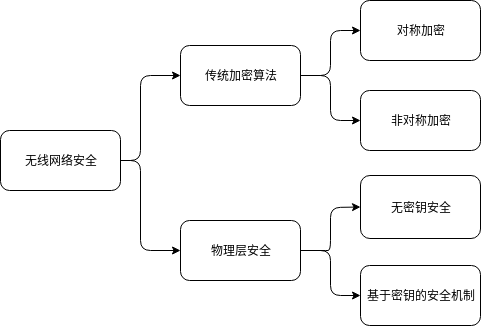
\includegraphics[width=0.9\textwidth]{images/wireless-network-security} 
    \caption{无线网络安全}
    \label{wirelss-network-security}
\end{figure}

本文研究无线信道密钥生成,即利用无线信道的随机性来生成密钥。和公钥体系利用数论问题保证安全性不同,无线密钥生成的安全性基于信息论。因为它基于无线信道的随机性\cite{ahlswede1993common}\cite{maurer1993secret},并且不需要借助其他用户的信息。以上所提及方法的优缺点列在表\ref{comparison-different-schemes}。

\begin{table}[]
    \begin{tabular}{|l|l|l|l|l|}
    \hline
    方法 & 描述 & 实现复杂度 & 优点 & 缺点 \\ \hline
    对称加密 & 合法通信双方用对称密钥加密数据 & 易实现 & 算法复杂度低 & 提前协商会话密钥;计算安全性 \\ \hline
    非对称加密 & 合法通信双方使用一对公私钥协商会话密钥 & 易实现 & 可用于协商会话密钥 & 计算安全性;依赖PKI;不适于低功耗设备 \\ \hline
    无密钥安全 & 合法通信双方通过设计编码和信道特性避免泄露信息 & 实现复杂 & 信息论安全;无需密钥的安全传输 & 依赖窃听者的CSI \\ \hline
    基于密钥的安全机制 & 合法通信双方利用信道的随机性生成密钥 & 易实现 & 信息论安全;轻量;无需第三方参与 & 受限于信道特性本身 \\ \hline
    \end{tabular}
    \caption{不同方法的比较
    \label{comparison-different-schemes}}
\end{table}

1993年Maurer等人理论上提出密钥生成\cite{ahlswede1993common}\cite{maurer1993secret}。密钥生成的模型如图\ref{}所示。图\ref{}中Alice和Bob需要建立一个安全的加密通道,窃听者Eve与Alice相距d厘米,并监听了所有传输过程。Alice、Bob和Eve可以分别接收到信号$X^n = (X_1, ..., X_n)$,$Y^n = (Y_1, ..., Y_n), Z^n = (Z1, ..., Z_n)$。Alice和Bob在公共信道上交换消息s,Eve同样可以接收到消息s。对任何$\epsilon > 0$和足够大的$n$,如果存在$K^A = g_A(X^n, s)$和$K^B = g_B(Y^n, s)$使得密钥生成体系满足

\begin{eqnarray}
    Pr(K^A \neq K^B) < \epsilon \label{keyrate1} \\
    \frac{1}{n}I(K^A; s, Z^n) < \epsilon \label{keyrate2} \\
    \frac{1}{n}H(K^A) > R - \epsilon \label{keyrate3} \\
    \frac{1}{n}log[\mathcal{K}] < \frac{1}{n}H(K^A) + \epsilon \label{keyrate4}
\end{eqnarray}

那么式中R即可达密钥速率,其中$I(\cdot)$表示互信息,$\mathcal{K}$表示密钥key的字母表。公式\ref{keyrate1}表示Alice和Bob生成相同密钥的可能性;公式\ref{keyrate2}表示通过公共信道传输消息,不会泄露给窃听者Eve,从而保证密钥安全性;公式\ref{keyrate4}确保密钥是均匀分布。最大可达密钥速率可以用密钥容量定义,

\begin{equation}
    C_K = min[I(X;Y), I(X, Y|Z)]
\end{equation}

目前已经有一些研究工作实现上述理论。1995年第一个实际的密钥生成协议被提出\cite{hershey1995unconventional},之后陆续出现大量研究无线密钥生成的相关工作。\citet{WangSurvey}的第四章从信息论角度阐述了无线密钥生成。\citet{WangSurvey}将信道探测和量化合并为一个步骤来研究。\citet{zeng2015physical}介绍了密钥生成技术存在的机遇和挑战,但是未涉及到具体实现细节。尽管\citet{ren2011secret}总结了一些密钥生成方法,比如基于接收信号强度(RSS)和基于信道相位的方法,但是由于之后密钥生成方法和技术迅速发展,所以仍然需要对密钥生成方法进行梳理。本文会对密钥生成技术做一个完整的文献综述。同时,本文会对密钥生成技术的未来发展提出相关建议。

\section{研究内容和方法}

无线信道密钥生成协议通常包含四个步骤,信道探测、特征量化、信息调和以及隐私放大:

\begin{itemize}
    \item \textbf{信道探测}。信道探测是测量无线信道并提取无线信道特征的过程。通信双方互相收发导频信号,并从接收到的导频信号中提取信道特征。
    \item \textbf{特征量化}。特征量化是将无线信道特征通过预处理、归一化、量化等操作得到比特流的过程。由于提取的无线信道特征受到接收端增益等参数的影响,所以需要预处理、归一化等操作来使得双方探测的信道特征更加相近。之后,再量化成比特流。
    \item \textbf{信息调和}。信息调和是利用无线信道特征作为随机密钥源并结合合理可靠的交互协议生成会话密钥的过程。通信双方在探测信道之后,量化信道得到密钥,通过公共信道的交互协议去除密钥中的不一致比特,得到完全一致的会话密钥。
    \item \textbf{隐私放大}。隐私放大是进一步提高密钥随机性和可靠性、去除密钥中信道相关信息的过程。通过单向哈希函数等方法,可以移除密钥中隐藏的信道信息,进一步提高密钥的安全性。
\end{itemize}

本文基于GNURadio软件无线电开发平台,实现一种TDD/FDD下低时延宽带无线信道密钥生成系统。本文系统信道探测部分分为两种模式,一种TDD模式,另一种FDD模式,并研究两种模式下的信道互易性、密钥安全性等,设计TDD模式和FDD模式下低时延的会话密钥协商技术。无论是TDD还是FDD,其核心都是通信双方在相干时间内获取对端发射的导频信号,并从接收的导频信号中分析和提取信道特征。两种模式除了信道探测部分不同,其余三部分均比较相似。

TDD模式和FDD模式的主要不同点是收发导频信号的机制不同。TDD模式下,通信双方工作在同一频率,相干时间内,两个发送端发射的电磁波经管相同的信道衰落;FDD模型下通信双方工作在不同频率,收发导频信号几乎发生在同时。由于合法通信双方的通信信道在空间上唯一性,所以即便第三方窃听者监听到任意一方发送的导频信号,也无法分析出通信双方之间的CSI信息,以此保障密钥的安全。

无论是TDD模式还是FDD模式,通信双方提取出CSI之后的主要过程是相似的:量化、调和。由于无线信道的短时互易性,通信双方的CSI是相近的,在量化之后得到的比特流也是相似的,但是由于信道在探测时隙内发生变化以及周围环境中的干扰等各种因素,双方提取的密钥又是不完全一致的。因此需要进一步调和,去除不一致比特或者纠正错误比特。调和之后,通信双方会获取一致的比特流,为了进一步去除比特流中的信道信息,进行隐私放大得到最终的会话密钥。

GNURadio是软件无线电开发平台,被广泛应用于音频处理、移动通信、卫星追踪、GSM网络等计算机软件\cite{Blossom2004GNU},用户可以在GNURadio平台上设计、仿真以及部署高性能无线电的软件无线电系统。本文基于GNURadio软件无线电开发平台和USRP N210硬件,设计TDD/FDD下低时延宽带无线信道密钥生成系统,并验证生产环境下无线密钥生成技术的可靠性和安全性。

在现有关于无线密钥生成技术的研究中,无线密钥生成技术的理论和仿真居多,在实际生产环境中实现并验证的研究并不多见。本文基于GNURadio软件无线电平台,设计和开发了TDD/FDD模式下低延迟无线密钥生成系统,并在不同场景下采集数据,通过分析CSI的相关性、信道随机性、密钥随机性、信息泄露率等四种指标,充分验证无线密钥生成技术在实际环境中使用的安全性和可靠性。

\section{本文主要内容与章节安排}

本文主要研究无线信道密钥生成技术及其实际应用。文章先介绍了无线信道密钥生成技术的研究背景,并概述国内外无线信道密钥生成技术的研究现状,在现有研究基础上,基于GNURadio软件无线电平台,设计和开发TDD/FDD模式下低延迟无线密钥生成系统,系统达到todo的密钥生成速率,平均每次密钥协商过程todo秒,并提出相应的系统性能评估指标,在多种场景下评估系统性能并分析系统优缺点。

\subsection{本文主要内容}

本文完成的主要工作包括:

\begin{itemize}
    \item(1)分析无线密钥生成技术的意义和背景,介绍无线密钥生成技术的国内外研究现状以及相关问题
    \item(2)基于无线密钥生成技术的理论,设计完整的无线密钥生成技术方案,搭建TDD/FDD无线密钥生成系统。
    \item(3)基于TDD/FDD无线密钥生成系统,研究不同场景下无线密钥生成系统的安全性和可靠性,通过多次实验分析通信参与者CSI的相关性、无线信道随机性、密钥的随机程度、信息泄露量,支撑无线密钥生成技术的实际应用意义。
    \item(4)todo 射频指纹?
    \item(5)todo 通过某些技术提高互易性?
\end{itemize}

\subsection{本文章节安排}

根据以上研究内容,本文分为todo章,具体章节安排如下:

todo

\chapter{无线密钥生成系统的理论基础}

本章节主要介绍无线密钥生成系统的理论基础。无线密钥生成系统的本质是利用无线信道的短时互易性、时空唯一性进行密钥生成的工作,在信道探测之后,量化生成的CSI,并进一步调和和隐私放大。另外本章介绍了系统生成密钥的评估标准,通过CSI相关性、信道随机性、密钥随机性和信息泄漏率等四个方面评估系统生成密钥的可靠性和安全性。

\section{无线信道特性}

\subsection{无线信道的短时互易性}

在TDD系统的上下行链路中,假设通信双方Alice和Bob以及窃听者Eve。在相干时间内,Alice和Bob互相发射的信号经过相同的信道衰落,因此由此估计出的信道具有互易性。

在图\ref{wireless-channel}中,Alice和Bob之间上下行链路的频率响应分别为$H_{ab}(t)$和$H_{ba}(t)$,相干时间内有$H_{ab}(t) = H_{ba}(t)$。假设在一次信道探测过程中,探测时隙为$\Delta t$,相干时间$\tau$内,Alice和Bob分别测量信道为$\tilde{H_{ba}(t)}$和$\tilde{H_{ab}(t)}$,当$ \Delta t < \tau $时有,

\begin{equation}
    H_{ba}(t) \approx H_{ab}(t + \Delta t)
\end{equation}

即双方探测的信道是近似相同的,因此通信双方可以通过利用无线信道的短时互易性来探测信道,进而结合其他协议生成相同的一致密钥。

同时,由于射频端的非线性特性、信道估计引入的误差、信道的时变性等因素\cite{guillaud2005practical},通信双方对信道的探测结果会有波动性差异:

\begin{itemize}
    \item 器件非线性。射频器件的非线性会导致I/Q路不平衡,如图\ref{iq_imbalance}所示,IQ不平衡会直接影响信号的发射和接收。在TDD系统中,收发两端的IQ不平衡会给上下行信道估计的互易性带来损失。
    \item 信道时变性。在相干时间内,无线信道具有短时互易性。但是由于无线信道的时变性,当双方探测信道的时隙超过信道相干时间,上下行信道估计结果会出现一定差异。
    \item 信道估计引入的误差。在基于导频的信号估计中,通过接收的导频信号和发射的导频信号做数学运算估计信道的频率响应,算法原理是通过最小化均方误差来估计信道,因此算法本身具有一定误差。
    \item 其他。另外,还有上下行链路的加性噪声也会对接收的信号有加性影响,不同频率子载波也会导致上行链路的差异等等。
\end{itemize}

\begin{figure}[htbp!]
    \centering 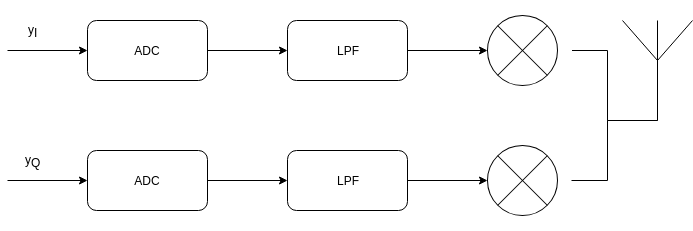
\includegraphics[width=0.9\textwidth]{images/iq_imbalance} 
    \caption{发射机存在的IO不平衡}
    \label{iq_imbalance}
\end{figure}


目前已经有相关工作研究如何对信道互易性的损失进行补偿,比如信道预测技术对信道互易性进行补偿,其原理是利用信道探测数据本身对未来时间的信道数据做出预测\cite{heidari2010adaptive}。另外基于信道互易性的MIMO预处理技术也可以一定程度上提高信道互易性,进而提高密钥一致性。针对IQ不平衡致使的信道互易性损失,可以估计系统中的不平衡参数,使相邻子载波的均方误差最小\cite{tubbax2005compensation}。

\subsection{无线信道的时空唯一性}

\begin{figure}[htbp!]
    \centering 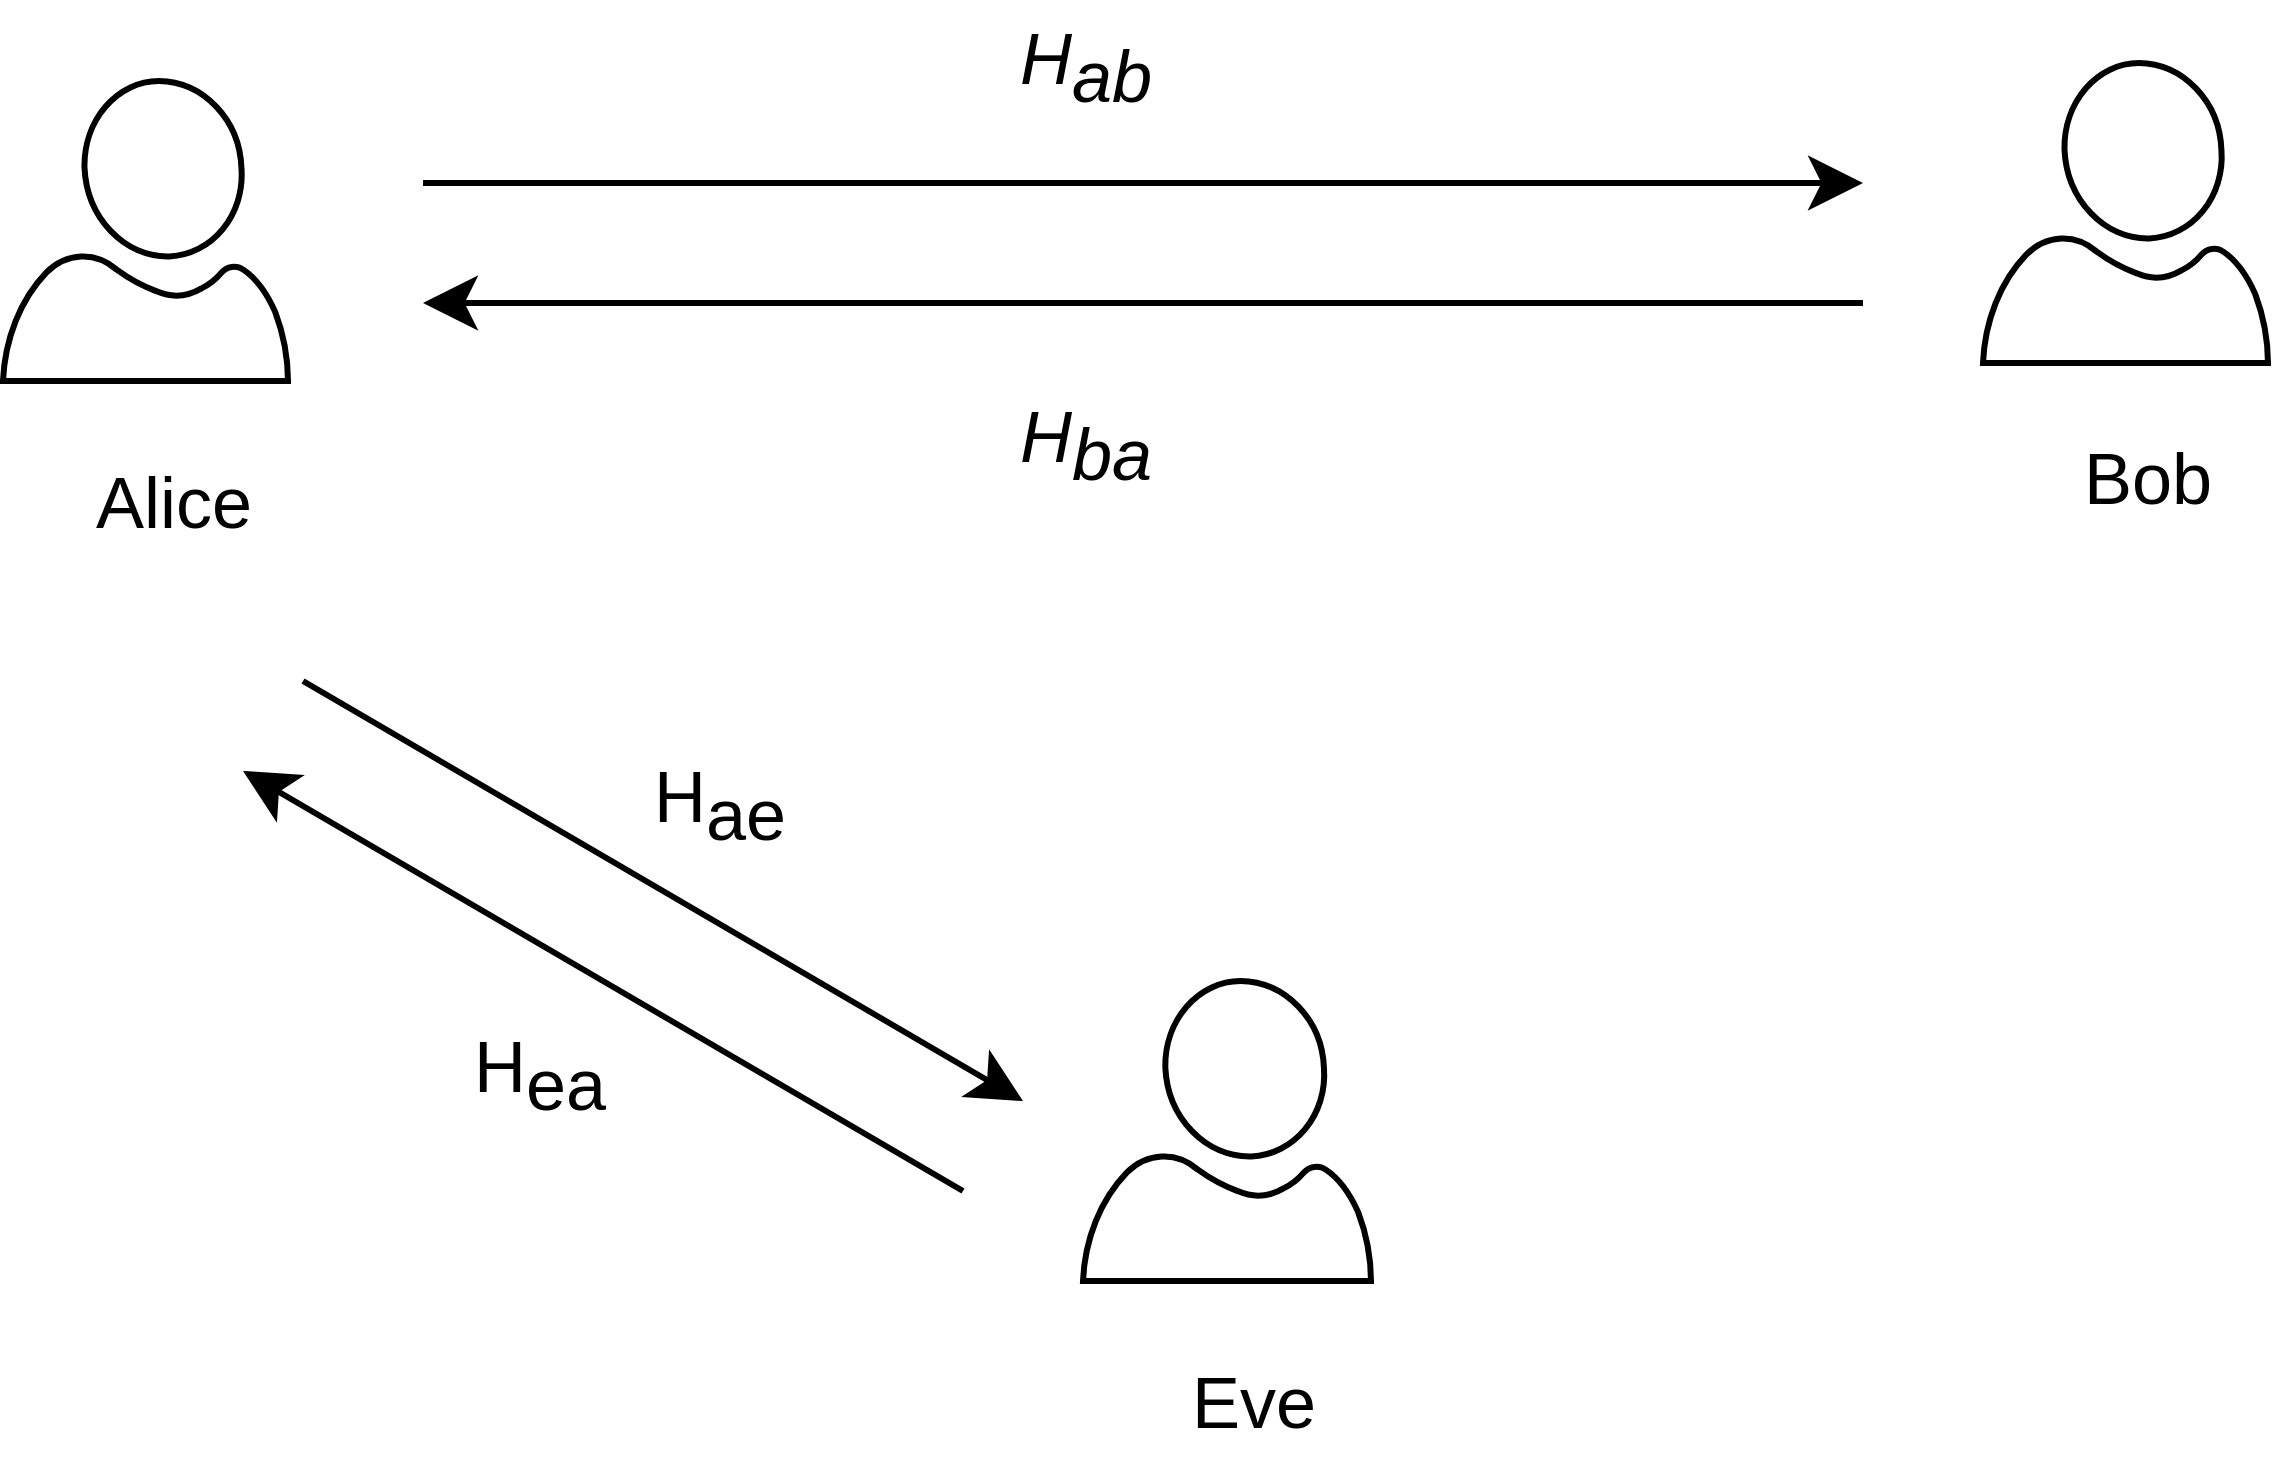
\includegraphics[width=0.9\textwidth]{images/channel} 
    \caption{无线通信信道}
    \label{wireless-channel}
\end{figure}

如图\ref{wireless-channel}所示,在某时刻t,通信双方Alice和Bob互相发射导频信号,在相干时间内,经管相同的多径信道衰落,对于窃听者Eve来说,无论是窃听来自Alice还是Bob的发射信号,其信道衰落都不同于Alice和Bob之间的信道衰落。在相干距离d(半波长)以外,Eve接收信号经历的多径衰落与Bob接收信号的多径衰落不再相关。除非攻击者在物理空间上靠近任意合法通信双方,否则无法分析出通信双方的CSI\cite{sasaoka2009secret}。

\subsection{无线信道的时变特性}

% 参考 3.1.1

信道衰落分为两类,大尺度衰落和小尺度衰落。大尺度衰落包括路径损耗和阴影损耗,在长距离传输(上百米)中,信号强度会发生变化。路径损耗指空间传播中电磁波的损耗,阴影损耗指在电磁波在传输过程中,受到遮挡物影响产生阴影效应,导致场强变化。通常用自由空间模型、Hata-Okumura,模型等来描述大尺度衰落。

小尺度衰落通常反应在短距离范围内信号幅值的变化中,通常符合瑞利分布、莱斯分布,小尺度衰落分为快衰落信道和慢衰落信道,快衰落信道又分为空间选择性快衰落信道、时间选择性快衰落信道、频率选择性快衰落信道。小尺度衰落反应无线信道的多径和时变,在无线通信中,通信双方之间信号经过的物理路径比较复杂,会收到多径的影响,可以将多径衰落信道建模成时变脉冲有限响应滤波器(FIR),即,

\begin{equation}
    h(\tau, t) = \sum_{l = 1}^{N(t)} a_k(t) \sigma(\tau - \tau_k(t))
\end{equation}

其中,t时刻,多径分量个数为$N(t)$,$a_k(t)$表示t时刻第l条路径信号幅度,$\tau_k(t)$表示t时刻第l条路径的延迟。

在一次信道探测过程中,若探测间隙大于信道的相干时间,接收信号经历快衰落过程,即时间选择性衰落。若信号带宽大于信道的相干带宽,接收信号经历频率选择性衰落,接收信号会产生符号间干扰(ISI)。


\section{密钥生成流程}

本文基于无线信道密钥生成技术设计的系统主要分为四个阶段,信道探测、特征量化、信息调和,整体架构如图\ref{whole_structure}所示。其中,Alice和Bob是合法通信双方,Eve是第三方窃听者。信道探测阶段是无线信道传输导频信号,信息调和阶段是通过公共信道传输调和信息。

\begin{figure}[htbp!]
    \centering 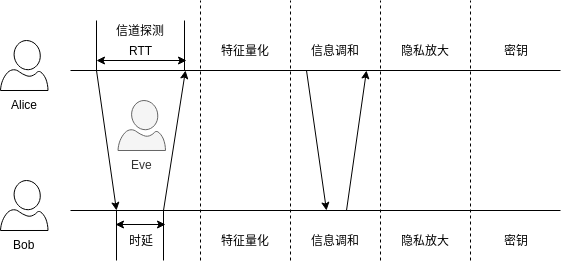
\includegraphics[width=0.9\textwidth]{images/whole_structure} 
    \caption{无线密钥生成流程的整体架构}
    \label{whole_structure}
\end{figure}

\subsection{信道探测}

在一个单入单出线性系统中,设脉冲响应函数为$g(k)$,根据维纳-霍夫方程的离散形式,发射信号$x(k))$和$y(k)$之间的相关函数为,

\begin{equation}
    R_{xy}(\tau)  = \sum_{j=0}^{\infty} g(j) R_x(\tau-j)\Delta t
\end{equation}

同时,M序列的自相关函数为,

\begin{equation} \label{m_self}
    R_m(\tau) = \left\{
  \begin{aligned}
  &1, &\tau = 0, N, 2N, ... \\
  &-\frac{1}{N}, &wherelse \\
  \end{aligned}
  \right.
\end{equation}

因此,当发射信号x(k)为M序列时,即$x(k) = m(k)$时,有,

\begin{equation}
    R_{ym}(k) = \sum_{j=0}^{N-1} \tilde{g}(j)R_m(k-j)\Delta t
\end{equation}
\begin{equation}
    R_{ym}(k) = \frac{(N+1)\Delta t}{N} \tilde{g}(k) - \frac{\Delta t}{N} \sum_{j=0}^{N-1} \tilde{g}(j)
\end{equation}
  
\begin{equation}\label{eq1}
    \tilde{g}(k) = \frac{N}{(N+1)\Delta t} [R_{ym}(k) + c]
\end{equation}

其中,

\begin{equation}
  R_{ym}(k) = \frac{1}{N}\sum_{j=0}^{N-1}m(j-k)y(j)
\end{equation}

工程上,

\begin{equation}
  c=-R_{ym}(N_P - 1)
\end{equation}
  
在TDD/FDD系统中,用户Alice和Bob互相发送导频信号帧$m(t)$作为导频信号。设$h_{ab}$代表Alice到Bob信道的频率响应,$h_{ba}$代表Bob到Alice信道的频率响应。那么,

Alice检测的时域信号为,

\begin{equation}
    y_{ba}(t) = m(t) * h_{ba}(t) + n_{ba}(t) 
\end{equation}

Bob检测的时域信号为,

\begin{equation}
    y_{ab}(t) = m(t) * h_{ab}(t) + n_{ba}(t)    
\end{equation}

因此Bob通过式(\ref{eq1})估计信道,

\begin{equation}
    \tilde{h}_{ab}(k) = a\sum_{j=0}^{N-1}m(j-k)y_{ab}(j)
\end{equation}
  
同理,Alice通过式(\ref{eq1})估计信道,
  
\begin{equation}
    \tilde{h}_{ba}(k) = a\sum_{j=0}^{N-1}m(j-k)y_{ba}(j)
\end{equation}
  
其中,a为常数,

\begin{equation}
    a = \frac{2-N_p}{(N + 1)\Delta t}
\end{equation}

\subsection{预处理}

在步骤信道探测中,通信双方分别通过导频信号估计探测时隙$\tau$内的脉冲响应$\tilde{h}_{ba}$和$\tilde{h}_{ab}$,并进行快速傅里叶变换得到信道频率响应$\tilde{H}_{ba}$和$\tilde{H}_{ab}$。由于在探测过程中,无线信道测量结果会受到环境噪声、射频器件的非线性等因素影响,因此通常会进一步预处理来提高信道的互易性和消除数据冗余。

\begin{equation}
    \tilde{H}_{ba} = Pre(FFT(\tilde{h}_{ba}))
\end{equation}
\begin{equation}
    \tilde{H}_{ab} = Pre(FFT(\tilde{h}_{ab}))
\end{equation}

其中,$Pre$表示预处理函数,$FFT$表示快速傅里叶变换。

\subsection{特征量化}

目前有多种量化策略,常用的有单门限量化、多门限量化、自适应门限量化等。

文献\citet{aono2005wireless}采用如图\ref{single_quantization}所示的单门限量化,量化阈值取RSSI(Radio Signal Strength Indicator)平均值,可以带来比较高的密钥一致率,但是测量值在阈值附近时容易量化错误,并且由于量化精度不高,在信道变化缓慢时,生成密钥容易出现大量连续0比特和1比特长串。

\begin{figure}[htbp!]
    \centering 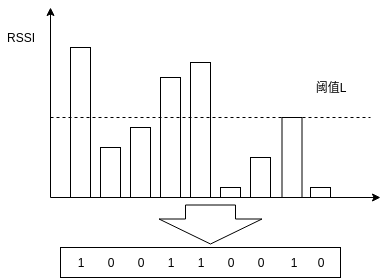
\includegraphics[width=0.9\textwidth]{images/single_quantization} 
    \caption{单门限量化}
    \label{single_quantization}
\end{figure}

文献\citet{mathur2008radio}采用如图\ref{two_quantization}所示双门限量化,将门限$L^+$和$L^-$之间的值舍弃,将$L^+$以上的值量化为1,将$L^-$以下的值量化为0,通信双方会在公共信道上交互传输未舍弃比特位的索引信息,因此第三方窃听者只有可能得知哪些比特被使用而无法得知被量化成0还是1,但是会降低密钥生成速率。

\begin{figure}[htbp!]
    \centering 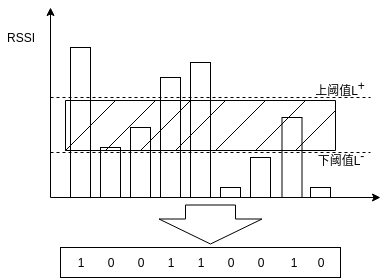
\includegraphics[width=0.9\textwidth]{images/two_quantization} 
    \caption{双门限量化}
    \label{two_quantization}
\end{figure}

文献\citet{patwari2009high}通过多次测量表明双门限量化每次会丢失5\%至27\%的比特数,并提出多比特自适应量化方法。文献\citet{yasukawa2008secret}使用多级量化,先将RSSI根据大小排序,然后分割成等间隔的$N = 2^m$块,m是量化比特数,并且通常$N \leq log_2^{maxValue}$,这样每个量化阶值的出现率是相同的。

通常多比特量化之后,会进一步编码成对应阶数格雷码。格雷码的特性是,相邻位置的格雷码只有一个位置的比特不同,因此使用格雷码可以提高通信双方的密钥一致率。无论是上述哪种量化方法,都避免不了密钥生成率和密钥一致性之间的矛盾。量化阶数越高,量化比特数越多,密钥生成率越高,但误差影响较大,密钥一致率降低;量化阶数越低,量化比特数越少,密钥一致率越高,但是密钥生成速率越低。

本文使用均匀量化的方法。在一次密钥生成过程中,Alice和Bob分别探测信道、预处理得到CSI。先对CSI降采样,以降低密钥泄漏率\cite{linning2019investigation}。同时,量化可以降低噪声的影响\cite{wang2015survey}。设量化时CSI最大值为$m_{max}$,量化阶数为R,量化前的值为m,量化后的值为q,将CSI归一化后按照式\ref{quantization_formula}均匀量化,得到离散的采样值,采样值对应比特数即量化阶数,本文量化阶数为3。密钥的生成速率与量化阶数成正比,通信双方的密钥一致率与量化阶数成反比。因此可以根据信噪比去调整量化阶数以得到较为均衡的密钥生成速率与一致率。量化之后的采样值需要进一步格雷编码降低密钥的不一致率。然后进行8b10b编码,过程如图\ref{quantization}所示。

\begin{equation} \label{quantization_formula}
    q = \frac{2^R * m}{m_{max}}
\end{equation}

\begin{figure}
    \centering
    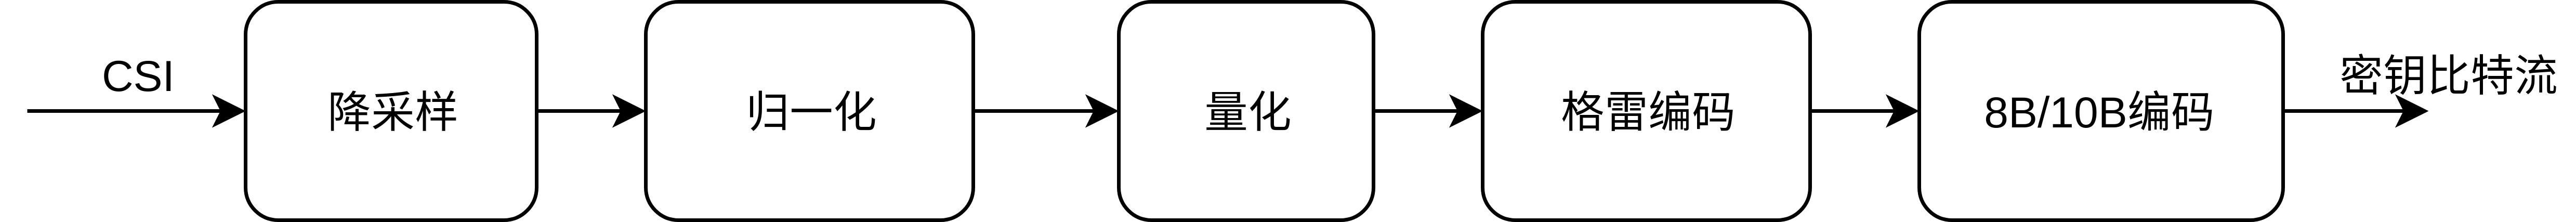
\includegraphics[width=0.9\textwidth]{images/quantization}
    \caption{量化}{} % Quantization.
    \label{quantization}
\end{figure}

\subsection{信息调和}

信息调和是在公共信道对不完全一致的密钥信息协商。由于短时信道互易性,所以通信双方分别通过上述步骤提取出的密钥是近似的,但是由于信道在探测的时隙内发生变化、环境中的干扰以及硬件指纹等各种因素,双方提取出的密钥又是不完全一致的。因此需要进一步调和。

信息调和通常基于Caseade协议\cite{Kitano2007A}或者纠错编码,比如 Turbo 码,BCD 码,LDPC 码等\cite{peng2018securing}。本文使用两种方式调和生成密钥。假设通信双方Alice和Bob,量化之后提取的比特字符串为$key1$和$key2$。

如果通过CRC校验码去除不一致比特,那么Alice将比特字符串$key1$分组并计算CRC校验码,将冗余部分码字发送给Bob。Bob进行同样分组,并根据Alice发送过来的冗余部分码字去除不一致的组。Bob再将检验结果回发给Alice,Alice根据校验结果去除不一致的组。最终双方可以得到一致的会话密钥。使用CRC校验码的调和过程如图\ref{crc}所示。

\begin{figure}
    \centering
    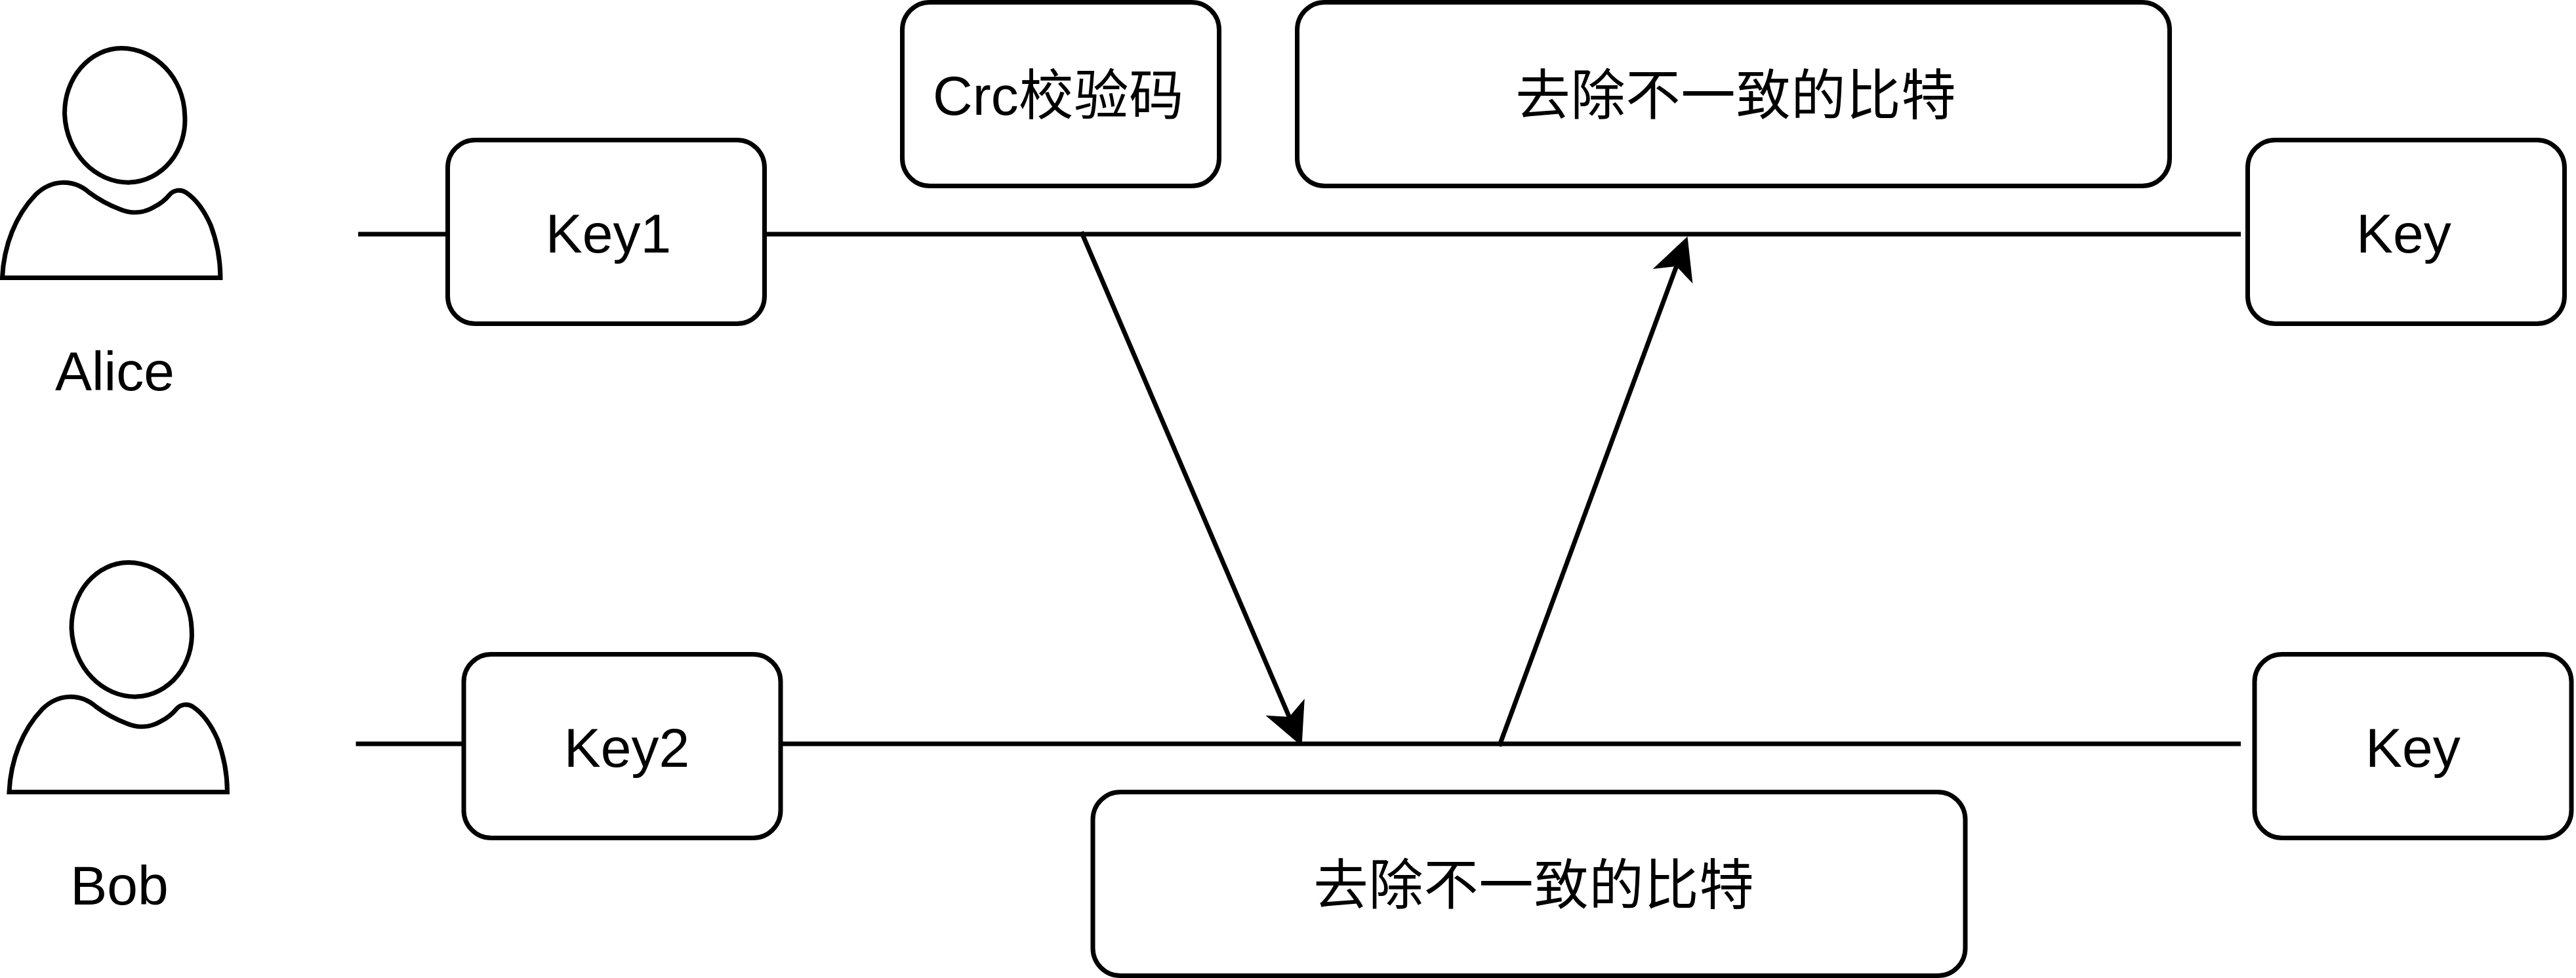
\includegraphics[width=0.9\textwidth]{images/crc}
    \caption{信息调和}{} % Crc Reconciliation
    \label{crc}
\end{figure}

% todo 纠错解码着一块还可以写的更加详细一点
除了通过CRC校验码去除不一致比特,Alice先将会话密钥进行纠错编码,再和key1异或,然后发送给Bob,Bob再次和key2异或,之后通过纠错解码器纠正错误比特位得到会话密钥key'。使用纠错码的过程如图\ref{error_correcting_code}所示。

\begin{figure}
    \centering
    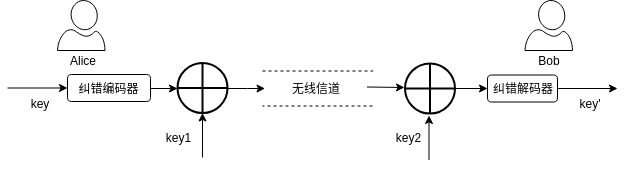
\includegraphics[width=0.9\textwidth]{images/error_correcting_code}
    \caption{纠错码}{} % Crc Reconciliation
    \label{error_correcting_code}
\end{figure}

% TODO
\subsection{隐私放大}

\section{无线信道密钥的评估标准}

本文为评估无线密钥生成系统性能,通过CSI相关性、信道随机性、密钥随机性和信息泄漏率等四个方面评估系统生成密钥的可靠性和安全性。

\subsection{CSI相关性}

本文通过皮尔逊相关系数计算CSI相关性,假设通信系统中,合法通信双方Alice和Bob信道探测结果为$\tilde{H}_{ba}$和$\tilde{H}_{ab}$,窃听者Eve探测结果为$\tilde{H}_{ae}$。

那么Alice和Bob之间CSI相关性为,

\begin{equation}\label{equation_corr}
    Reprocity_{ab, ba} = \frac{E[(\tilde{H}_{ab}-\mu_{\tilde{H}_{ab}})(\tilde{H}_{ba}-\mu_{\tilde{H}_{ba}})]}{\sigma_{\tilde{H}_{ab}}\sigma_{\tilde{H}_{ba}}}
\end{equation}

为研究Eve窃听的CSI结果与合法信道的CSI结果的差异,计算Eve的CSI和Alice的CSI相关性,

\begin{equation}\label{equation_corr}
    Reprocity_{ab, ae} = \frac{E[(\tilde{H}_{ab}-\mu_{\tilde{H}_{ab}})(\tilde{H}_{ae}-\mu_{\tilde{H}_{ae}})]}{\sigma_{\tilde{H}_{ab}}\sigma_{\tilde{H}_{ae}}}
\end{equation}

其中,$\sigma_{\{.\}}$表示标准差,$E\{\cdot\}$表示期望。

理论上,在相干距离之外,

\begin{equation}
    Reprocity_{ab, ae} < Reprocity_{ab, ba}
\end{equation}

$Reprocity_{ab, ba}$越大表明合法通信双方信道互易性越好,CSI相关性越高,密钥一致率越高。$Reprocity_{ab, ba}$较低的原因可能是通信双方硬件指纹差异、信道环境糟糕等,可以使用一些预处理算法弥补互易性的损失。

$Reprocity_{ab, ae}$越小表明第三方可以窃听的信息越少,CSI相关性越低,密钥泄露更少。在相干距离(通常是半波长)以外,由于导频信号经过不同的信道衰落,因此Eve估计得到的CSI与合法信道的CSI相关性较低。在相干距离以内,由于物理距离上接近,Eve估计的CSI相关性较高,但是在实际环境中,窃听者无法如此靠近合法通信参与者。

\subsection{信息泄露率}

本文设计的密钥生成系统中,在信道探测、信息调和阶段,对第三方来说是完全透明的\cite{sahin2016secure}。设Alice、Bob和Eve对信道探测为$H_A$、$H_B$和$H_E$。则A和B之间信道的互信息为,

\begin{equation}
    I_k = I(H_A; H_B) = log_2^{\frac{\left|R_{AA}\right|\left|R_{BB}\right|}{\left|R_{AB}\right|}}
\end{equation}

其中, $\left|R_{xy}\right| = E\{H_x H_y^H\}$表示协方差系数。

存在eve时,alice和bob之间的互信息量为, 

\begin{equation}
  I_{sk} = I(H_A; H_B | H_E) = log_2^{\frac{\left|R_{AE}\right|\left|R_{BE}\right|}{\left|R_{EE}\right|\left|R_{ABE}\right|}}
\end{equation}

通过$I_{sk}$与$I_k$的比例来评估信息未泄露的比率,

\begin{equation}
  \eta = I_{sk} / I_k
\end{equation}

\subsection{随机性评估}

本文既评估了系统运行过程中的CSI随机性,也测试了生成密钥的随机性。

\subsubsection{CSI随机性}

CSI的随机性既有时域的变化,也有频域的变化。为了衡量CSI的随机性,本文采集了不同场景下的多组CSI,计算多组CSI的图像熵,用来衡量CSI的随机性。

使用二维快速傅里叶变换(2d-fft)的图像熵来表征信道的随机性。设计算得到的多组CSI归一化之后为矩阵$C_{MxN}$,M为CSI长度,N为采集的CSI组数。$C(x, y)$表示第i行第j列的值,那么对其做2d-fft计算,其2d-fft的矩阵为,

\begin{equation}
  F(u, v) = \frac{1}{MN}\sum_{x=0}^{M-1}\sum_{y=0}^{N-1} C(x,y) e^{-j2\pi(\frac{xu}{M}+\frac{yv}{N})}
\end{equation}


为了缩小差距,将$F$取In函数得到$L$,

\begin{equation}
  L(u, v) = log_e^{F(u, v)}
\end{equation}

再归一化到[0, 1]范围内得到,

\begin{equation}
  I(u, v) = \frac{L(u, v) - min{L}}{max(L) - min(L)}
\end{equation}

将[0, 1]区间分割成256等份,统计I(u, v)在各个区间的概率,计算I(u, v)的熵,

\begin{equation}
  H(u, v) = -\sum_{i=1}^{256} p_i log_2^{p_i}
\end{equation}

\subsubsection{密钥随机性}

本文使用NIST(National Institute of Standards and Technology,NIST)随机性测试来评估密钥的随机性\cite{bassham2010statistical}。NIST随机性测试通过多个维度测试密钥的随机性\cite{zaman2012review}。NIST官网包含了16项统计测试,每项测试会对给定比特序列做在随机性假设下的卡方检验,其将$\chi^2$值转换为随机性概率,即程序中的P值,表示随机性的可能性大小。表\ref{NIST-schemes}为NIST随机性测试的15项测试手段。如果P值大于0.01,则表示比特序列是随机的。

% 参考

\begin{table}[]
    \begin{tabular}{p{70pt}p{70pt}p{200pt}p{100pt}}
    \hline
    方法 & 参数要求 & 原理 & 不通过原因 \\ \hline
    频数检验 & N $\geq$ 100bits & 序列中1和0数目是否相近 & 说明1和0数目相差过多  \\ \hline
    块内频数检验 & N $\geq$ 100bits 子块 M > 0.01N & M位子块中1的个数是否接近m/2 & 至少某一个子块0、1比例不均衡 \\ \hline
    游程检验 & N $\geq$ 100bits 设定$\tau = \frac{2}{\sqrt{n}}$,用于判定是否频数检验 & 检验不同长度的游程总数是否符合随机序列的期望值 & 说明游程综述过大或者过小,即,序列中元素变化过快或者过慢  \\ \hline
    块内最长游程检验 &  & 检验序列中各个等长子序列中最长1游程的长度是否符合随机序列的期望值 & 检验序列中有太多的(成簇的)1 \\ \hline
    二元矩阵秩检验 & N $\geq$ 38MQ,行列M=Q=32 & 由检验序列的给定长度子序列构成序列,检验构造矩阵行或列之间的线性独立性 & 秩分布与相应的随机序列有一个大的偏离 \\ \hline
    离散傅里叶变换检测 & N $\geq$ 1000 & 使用频谱方法检验序列进行傅里叶变换后的尖峰高度是否超过某个门限值 & 太多傅里叶变换的尖峰高度超过门限值 \\ \hline
    非重叠子模块检验 & $ N \geq 10^6$  m={9, 10} & 使用一个m-bit窗口来搜索一个特定的m-bit模式,检验设置好的目标数据串的发生次数 & 存在无规则发布的模块 \\ \hline
    重叠子序列检验 & $N \geq 10^6$ m={9, 10} & 检测提前设置好的目标数据串发生的数目与非重叠子模块相似,不同之处在于发现目标模块后,窗口仅向后移动一位 & 在太多的目标数据串存在 \\ \hline
    Maurer通用统计检验 & & 检验序列是否可被无损压缩 & 序列可大幅度的被压缩 \\ \hline
    % Lempel-Ziv压缩检验 & $N \geq 10^6$ & 检验序列能够被压缩到什么程度 & 序列可以被很大程度压缩,说明非随机 \\ \hline % 在最新版本中已经被去除
    线性复杂度检验 & $N \geq 10^6$ & 检验各等长的子序列的线性复杂度是否符合随机序列期望值 & 子序列线性复杂度分布不规则 \\ \hline
    序列检验 & $ m < [log_2^N] - 2$ & 检验序列中m位可重叠子序列的每一种模式个数是否接近,对随机序列来说,m位可重叠子序列的每一种模式出现的概率应该相等。m=1时即1 & 序列中长度为m的可重叠子序列模式分布不均匀 \\ \hline
    近似熵检验 & $ m < [log_2^N] - 2$ & 看整个序列中所有可能的重叠的m-bit模式的频率,目的是将两相邻长度(m和m+1)的重叠子块的频数与随机情况下预期的频数相比较 & 序列有较强的规律性 \\ \hline
    累加和检验 & $N \geq 100bits$ & 最大累加与随机序列中具有的最大偏移相比较,应该接近0 & 说明序列早期或者晚期有过多1或者1 \\ \hline
    随机游动检测 & $N \geq 10^6$ & 看一个累加和随机游动中具有K个节点的循环个数 & 与预期背离 \\ \hline
    随机游动状态频数检验 & $N \geq 10^6 $ & 看累加和随机游动中经历的特殊状态的总数。检验目的即:判定随机游动中实际经历多个状态的值和预期值之间的偏离程度 \\ \hline

    \end{tabular}
    \caption{NIST测试
    \label{NIST-schemes}}
\end{table}

\subsection{密钥不一致率和密钥生成速率}

密钥不一致率(KDR,Key Disagreement Rate)指在调和之前,通信双方生成密钥的不一致比特占比。高KDR通常表示密钥生成协议的效率较低,甚至可能由于KDR较高导致错误比特数超过纠错码的纠错极限。基于RSS的密钥生成方法的KDR通常由无线信道的多径和时变决定\cite{jana2009effectiveness}。通过多天线可以提高KDR,因为多天线可以提供更多的互信息。在一个低信噪比(SNR)的环境中,由于信道估计的误差更大,所以KDR更低。

密钥生成速率(KGR,Key Generate Rate)可以用于表示系统生成密钥的效率,即平均每秒或者每次信道测量最终可以生成的密钥比特数。KGR越高,通信双方可以在短时间内建立会话密钥,达到较高通信效率。基于RSS的密钥生成方法通常KGR非常低,因为该方法需要平衡KGR、KDR。为了减少KDR,通常不得不将连续多个值当做一个比特处理,此外该方法的KGR收到瑞利衰减信道的幅度交叉率限制(level-crossing rate)。虽然过采样可以带来更高的信道相关性,但是却会导致密钥随机性降低\cite{mathur2008radio}。多天线系统可以带来几乎四倍于普通方法的密钥生成率\cite{zeng2010exploiting}。

\section{本章小结}

本章主要介绍无线密钥生成系统的理论基础,首先介绍无线信道的特征对无线信道密钥生成的影响,无线信道的短时互易性是无线密钥生成技术的基石,无线信道的时空唯一性决定第三方窃听信息的困难程度,无线信道的时变性会给无线密钥生成技术带来信道互易性上的损失。

之后详细阐述密钥生成流程的主要阶段,包括信道探测、预处理、特征量化、信息调和等无线信道密钥生成步骤的具体理论。信道探测用于获取CSI,预处理为了提高信道互易性,特征量化用于提取密钥比特流,信息调和步骤中协商生成一致的密钥比特流。

最后提出密钥生成系统性能的评估指标,包括CSI相关性、信息泄露率、CSI随机性、密钥随机性、密钥生成率、密钥不一致率等指标,用于衡量无线密钥生成系统的可靠性和安全性,CSI相关性和信息泄漏率表征第三方窃听信息的难度,CSI随机性和密钥随机性分别评估信道的随机性和密钥的随机性,密钥生成率表示系统生成密钥的效率,密钥不一致率表示通信双方调和前密钥的一致性。

\chapter{导频信号收发机设计}

在TDD通信系统中,考虑一对合法用户Alice和Bob在多径衰落信道工作,通信双方互相发送已知导频信号。在想干时间$\tau$内,通信双方发送的信号经过相同信道衰落到达对方。接收方由接收的导频信号与已知导频信号估计$\tau$这段时间内的信道。


% TODO 是否要加入纠错码这一块的详细设计和解释
% TODO 是否要加入GNURadio流式处理数据的pc和usrp之间的交互图
\section{导频信号}

\subsection{粗同步}
通信双方Alice和Bob均需要发送导频信号用于在通信过程中估计信道所用。在信道探测步骤中,为了可以更快的检测出指定信号,本文在导频信号首尾分别添加一段正弦波,如果检测到指定长度信号的首尾两端出现指定频率的正弦波,则说明该段信号是指定导频信号,将其存储供信道估计使用。

本文将以上步骤称为粗同步。设Alice发射导频信号为$Frame_a$,长度为$L_a$,$Frame_a$中首尾两端正弦波频率为$F_a$,检测阈值为$R_a$,fft长度为$L_d$,正弦波长度为$L_{sine_a}$。设Bob发射导频信号为$Frame_b$,长度为$L_b$,$Frame_b$中首尾两端正弦波频率为$F_b$,检测阈值为$R_b$,fft长度为$L_d$,正弦波长度为$L_{sine_b}$。GNURadio中处理数据的形式是高速实时数据流的形式,以Bob为例,接收数据流$S_a$对每段数据流输入,均会有数据流输出,本文对每L个长度的复数点做fft得到频域响应$H_{detect_a}$,并检查$ L_d - L_d / F_a $处幅值是否大于阈值$R_a$。即,在数据流$S_a$的位置i处计算,

\begin{equation}
    H_{detect_a} = FFT(S_a[i, i+L_d])
\end{equation}

若,

\begin{equation}
    H_{detect_a}[L_d - L_d / F_a] \geq R_a 
\end{equation}

则$S_a[i, i+L_d]$这段信号是指定$F_a$频率正弦波,说明这段信号前后存在需要检测的导频信号。为了确定导频信号在输入信号中的具体位置,需要判断距离相隔$L_a - L_{sine_a}$两个位置是否同时存在指定$F_a$频率的正弦波,如果这两个位置同时存在指定$F_a$频率的正弦波,那么这两个位置之间即需要检测的Alice发射的导频信号。即,在数据流$S_a$的位置$i$处和位置$i+L_a-L_{sine_a}$处计算,若,

\begin{equation}
    FFT(S_a[i, i+L_d])[L_d - L_d / F_a] \geq R_a 
\end{equation}

\begin{equation}
    FFT(S_a[i+L_a-L_{sine_a}, i+L_a-L_{sine_a}+L_d])[L_d - L_d / F_a] \geq R_a 
\end{equation}

那么,数据流$S_a$的位置$i$处和位置$i+L_a-L_{sine_a}$之间的数据即Bob需要检测得到的、Alice发射的导频信号,将这之间的信号保存下来。对于Alice来说,同理。

粗同步步骤出现在GNURadio检波程序中,相对于传统的相关检波,其时间复杂度更低。在检测过程中,会对每$L$长度的信号段做阈值检测,当出现前后两端正弦波并且间隔满足指定导频信号的要求时,即检测到导频信号,其过程如图\ref{detect_wave_algm}所示。

\begin{figure}
    \centering
    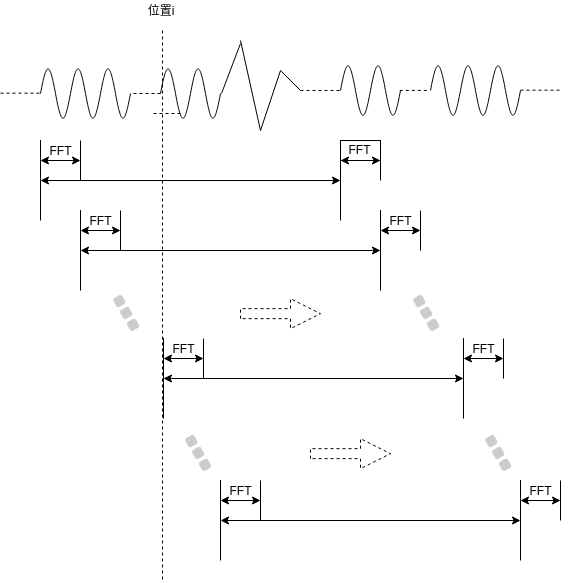
\includegraphics[width=0.9\textwidth]{images/detect_wave_algm}
    \caption{粗同步检波}{} % Crc Reconciliation
    \label{detect_wave_algm}
\end{figure}


\subsection{精同步}

在粗同步中,检波模块将检测到的导频信号转存到硬盘中,转存到硬盘的导频信号首尾两端是不完整的正弦波,首尾两端正弦波长度之和应该是$L_{sine_a}$,但是首部和尾部分别多长无法得知,因此需要进一步精确同步。

本文使用伪随机性序列(PN序列)作为精确同步和信道估计所用序列,由于m序列是PN序列中的一种,并且具有良好的自相关特性,所以本文使用m序列作为导频信号的主体部分。为了消除符号间干扰(Inter-Symbol-Interference,ISI)和载波间干扰(Inter-Carrier-Interference,ICI),在m序列后面添加循环前缀(Cyclic Prefix, CP)充当保护间隔,CP指的是将m序列的前面一部分复制到后段。

% TODO 加入仿真和实际测量中m序列自相关的图片
因为精同步发生在导频信号检测并转存之后,对实时性要求不高,因此本文利用m序列的自相关特性来精确切割导频信号。m序列的自相关函数是公式(\ref{m_self})所示周期性的二值函数,m序列的自相关函数时域上与冲激函数相近,在完全重合的周期点会出现波峰,并且随着m序列周期增加,m序列的随机性越好。设通信方转存的导频信号为$Rx$,包含的m序列理想情况为$m$,长度为$L_m$,第一段正弦波的完整长度为$L_{sine}$,那么可以遍历导频信号的起始一段,通过与已知原始m序列共轭相乘相加,求出波峰$Peak$并保存波峰位置i,

\begin{equation}
    Peak = max\{\frac{\sum_{k = i}^{L_m} \bar{m(k})\times Rx(i + k)}{L_m}) \}, i \in \{1, .., L_m + L_{sine}\}
\end{equation}

其中$\bar{\dot}$为取共轭。波峰$Peak$处对应的位置$i$就是精同步的结果,即m序列的起始位置,计算出m序列起始的精确位置,便可以进一步通过m序列或者其他数据段进行信道估计步骤。

图\ref{practical_pilot_m_seq}为系统转存的实际导频信号,其中包含第一段检波所用正弦波,以及m序列。通信方已知m序列原始信号如图\ref{m_seq}所示。图\ref{m_corr_practical}展示在实际系统中,转存信号中与已知m序列做相关的结果,其中根据波峰位置可以精确定位导频信号中m序列的起始位置。

\begin{figure}
    \centering
    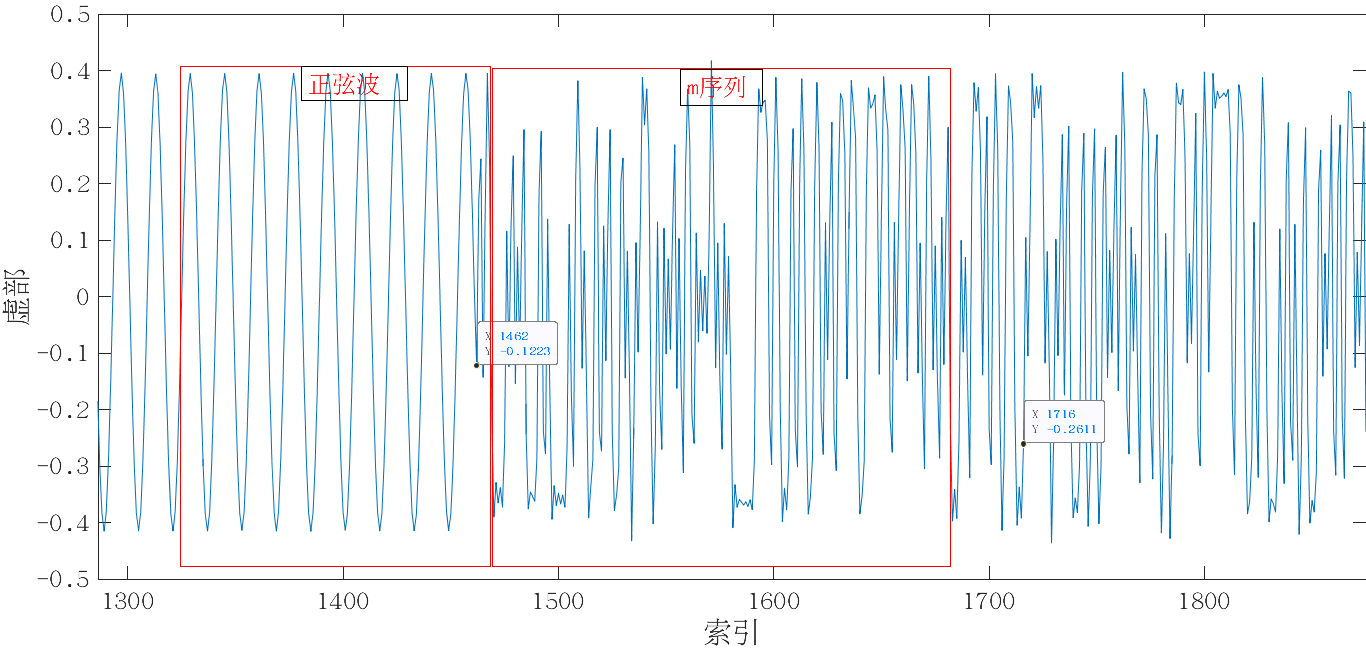
\includegraphics[width=0.9\textwidth]{images/practical_pilot_m_seq}
    \caption{实际导频信号中的m序列}{} 
    \label{practical_pilot_m_seq}
\end{figure}

\begin{figure}
    \centering
    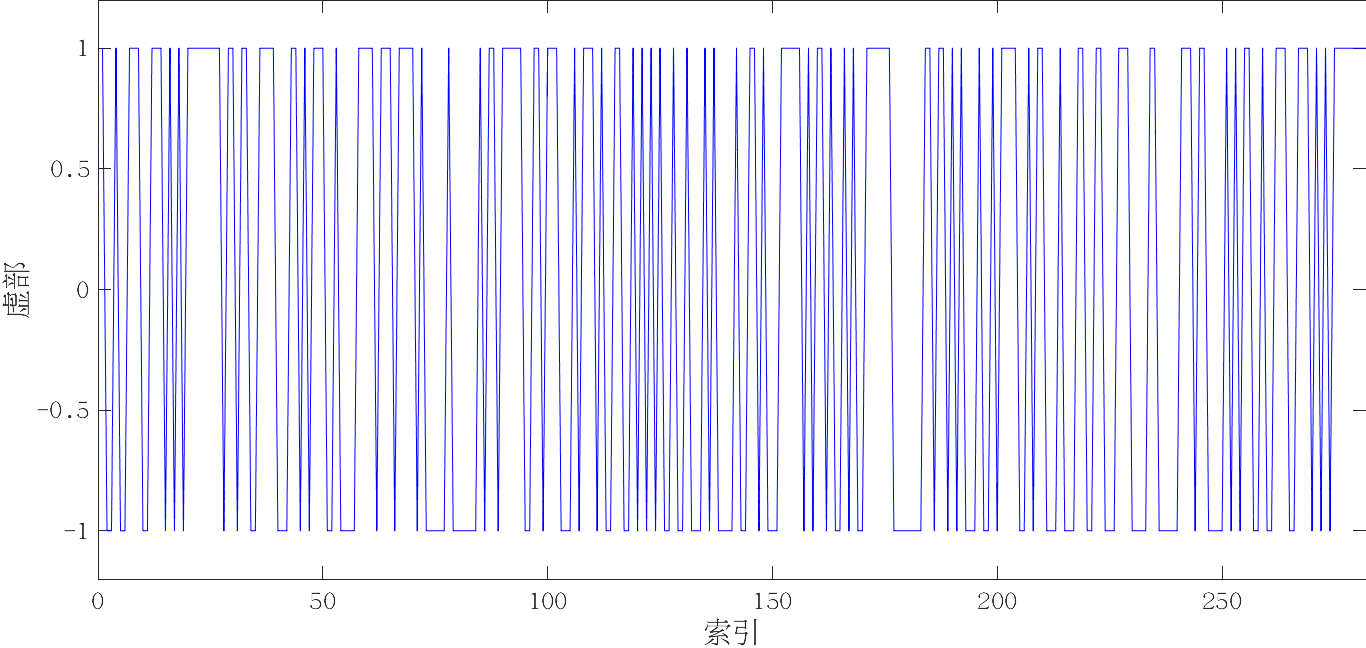
\includegraphics[width=0.9\textwidth]{images/m_seq}
    \caption{理想情况下的m序列}{} 
    \label{m_seq}
\end{figure}

\begin{figure}
    \centering
    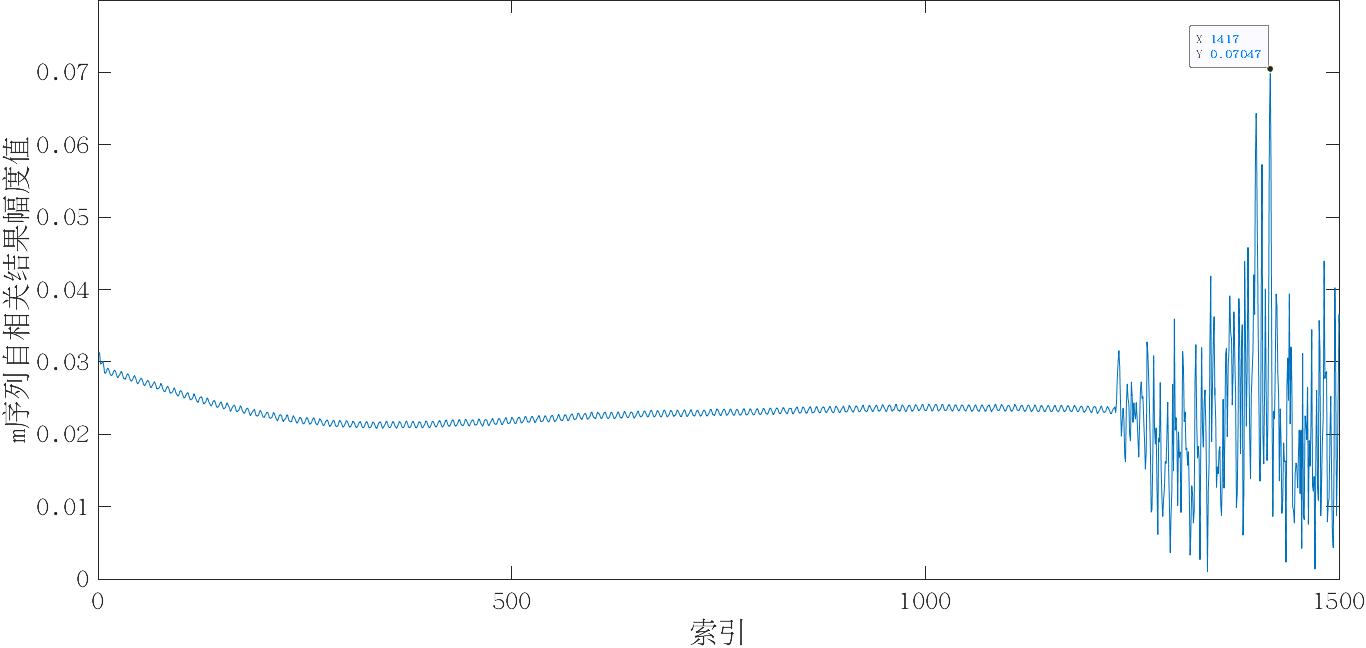
\includegraphics[width=0.9\textwidth]{images/m_corr_practical}
    \caption{理想和实际中m序列自相关}{} % Crc Reconciliation
    \label{m_corr_practical}
\end{figure}

\section{基于导频信号TDD收发系统设计}

本节阐述基于导频信号的TDD收发系统设计,从理论以及实现的角度详细介绍系统的构造。导频收发机是基于GNURadio搭建的,数据采集由USRP部分负责,USRP射频前端将数据转换到基带信号,并送入通用计算机中处理数据,实际上检波部分运行在计算机内,USRP将基带数据通过网口送入计算机内,计算机程序再去处理高速的数据流,并从中检测出导频信号。导频收发机是本系统最核心的部分,负责导频信号的发射、检测和转存。具体来说,由四个GNU Radio模块构成:导频序列输出模块、数据发射模块、数据接收模块、导频信号检测模块。以下会详细介绍四个模块的实现。

\subsection{导频序列输出模块}

导频序列输出模块,可以理解为导频信号生成的模块,为方便起见,事先已经生成好导频信号存储在文件中,该模块可以直接读取该文件并送到输出端口。这种类型模块在GNURadio称作输出模块,输出模块无输出端口、有输出端口。本文为其设计了一个控制信号,即\ref{file_source_roi}图中所示$Tx\_File$这个布尔量,该模块内部有一状态量$Tx\_File\_$表示该模块是否正在发射数据。

\begin{itemize}
    \item 当$Tx\_File$设置为$True$时,该模块会检查$Tx\_File\_$变量查看当前是否输出数据。如果正在输出数据,则不做任何事情;如果不在输出数据,则会读取导频信号文件并送出到输出端口,当数据输出完成时,将$Tx\_File\_$设置为$False$
    \item 当$Tx\_File$设置为$False$时,该模块的输出端口不会输出任何数据。
\end{itemize}

因此,上层程序只需要控制$Tx\_File$这个变量,就可以控制导频信号的发射与否。将$Tx\_File$置为$True$,则会向输出端口送出导频信号(如果当前模块不在发射的话),置为$False$,则会立即停止输出任何数据。

\begin{figure}
    \centering
    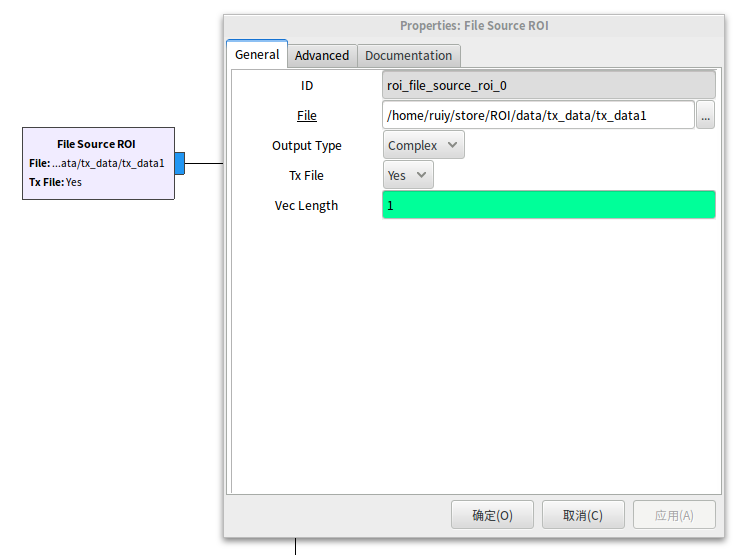
\includegraphics[width=0.9\textwidth]{images/file_source_roi}
    \caption{导频序列输出模块}{} 
    \label{file_source_roi}
\end{figure}

\subsection{数据发射模块}

% 参考 https://zhuanlan.zhihu.com/p/24217098

数据发射模块是直接使用了GNURadio自带的模块$UHD: USRP\quad Sink$,其属于GNURadio的$gr-uhd$系列,该模块用于将数据采样点送入USRP设备中,USRP设备会将其调制发射到指定频率。其参数如图\ref{usrp_sink}所示。

该模块实际是计算机端的控制平台,其实际执行是由USRP中的FPGA以及相关器件实现实现。该模块需要将基带数据通过USB口或者网口送入到USRP中去,如图\ref{usrp_sink_theory}所示为PC端与USRP端的交互。该模块属于计算机端的上层应用程序,使用C++或者Python编写,调用UHD驱动程序和系统调用,控制硬件接口的数据读写。PC与USRP的交互使用USB3.0或者以太网网口,目前大部分外设均使用USB3.0或者千兆以太网网口传输数据,来保证输出速率,满足实时性,USB3.0的速率可达到500MBps\cite{wei2016software}。

在发射数据时,进程从用户态切换到内核态,通过系统调用控制网卡或USB的读写。通过以太网网口或者USB口,将数据送入到USRP内部。USRP内部的处理分为三个部分。

\begin{itemize}
    \item 首先,发送控制模块和数字上变频模块(DUC)为了处理速度足够快,采用FPGA实现。发送控制模块控制USRP的发送时序。DUC模块用于基带数据上变频到中频\cite{xiong2015open}。
    \item 其次,中频数字信号经过DAC器件数模转换得到模拟域的数据,再进一步进行模拟域的信号处理
    \item 模拟域中,信号先经过低通滤波器得到更加平滑的信号,再与晶振信号相乘,将中频信号调制到指定射频频点,最后射频信号经过功率放大器发射出去。
\end{itemize}


\begin{figure}
    \centering
    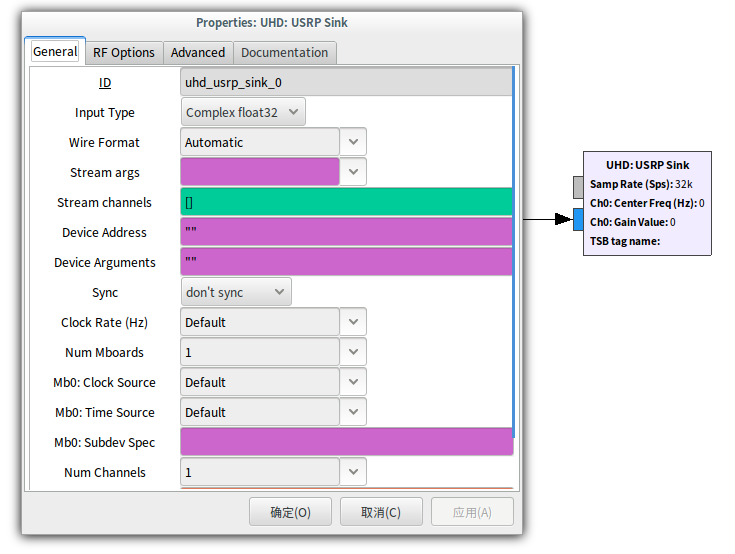
\includegraphics[width=0.9\textwidth]{images/usrp_sink}
    \caption{数据发射模块}{} 
    \label{usrp_sink}
\end{figure}

\begin{figure}
    \centering
    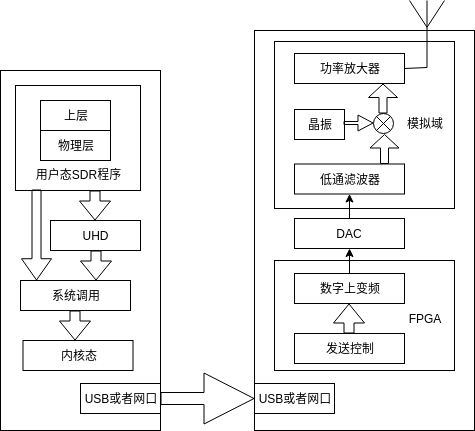
\includegraphics[width=0.9\textwidth]{images/usrp_sink_theory}
    \caption{数据发射时USRP内部示意图}{} 
    \label{usrp_sink_theory}
\end{figure}

\subsection{数据接收模块}

数据接收模块也是直接使用了GNURadio内置的模块,同属于$gr-uhd$的模块集,该模块和$UHD: USRP\quad Sink$作用相反,其作用是通过USB口或者千兆以太网网口从USRP中获取基带数据,并送入到输出端口。其参数如图\ref{usrp_source}所示。

\begin{figure}
    \centering
    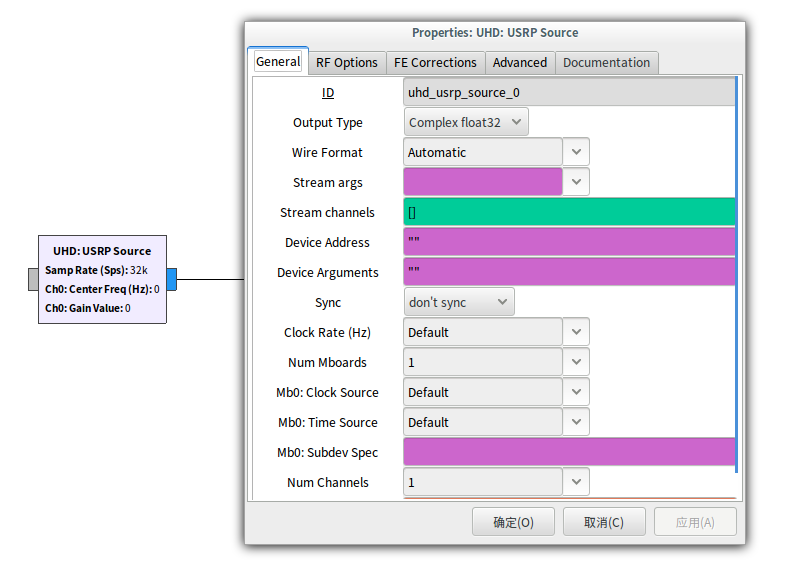
\includegraphics[width=0.9\textwidth]{images/usrp_source}
    \caption{数据接收模块}{} 
    \label{usrp_source}
\end{figure}

和$UHD: USRP\quad Sink$类似,该模块属于进程中的用户态部分,其在运行时会切换到内核态,并从与USRP相连接的以太网网口或者USB口读取高速数据。如图\ref{usrp_source_theory}所示为USRP在接收数据时与PC的交互。在接收数据时,USRP外设同样分为三个阶段处理信号,

\begin{itemize}
    \item 首先,信号经过低噪声放大器,避免将噪声放的过大。之后与晶振信号相乘,下变频到中频,再通过低通滤波器使得信号更加平滑。
    \item 其次,中频模拟信号通过ADC器件模数转换为数字信号。再进一步进行数字域的处理。
    \item 中频数字信号通过数字下变频,得到基带信号,再通过接收控制模块。为了速率保障,数字下变频模块和接收控制模块同样使用FPGA实现,接收控制模块控制USRP的接收行为。
\end{itemize}

USRP处理得到数字基带信号之后,通过以太网网口或者USB口,将数据送入PC中并触发中断,或者通知上层程序数据可读。PC中的上层程序陷入内核态,调用UHD驱动程序和系统调用从以太网网口或者USB口读取数据,然后返回用户态进一步处理数据。

\begin{figure}
    \centering
    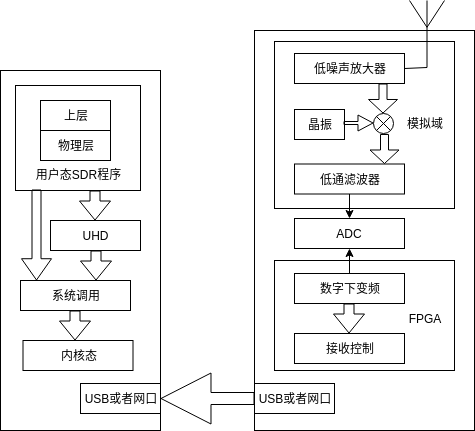
\includegraphics[width=0.9\textwidth]{images/usrp_source_theory}
    \caption{数据接收时USRP内部示意图}{} 
    \label{usrp_source_theory}
\end{figure}

\subsection{导频信号检测模块}

导频信号检测模块从数据接收模块中读取基带数据流,并按照上述粗同步的方式,通过fft检测指定间隔的两段信号是否为指定频率的正弦波,若是,则判断为需要检测的导频信号,将其转存到磁盘上,供之后信道估计使用。这种类型模块在GNURadio称作输入模块,输入模块无输出端口、有输入端口。

本文在设计该模块时提供了诸多模块参数,如图\ref{file_sink_roi}所示。其中各参数的意义为,

\begin{itemize}
    \item $Sine Freq$为该模块需要检测的导频信号首尾两端正弦波的频率
    \item $Threshold$为通过fft判断能量时所用阈值
    \item $FFT Size$为检波是所做fft长度
    \item $Rev-Send latency$为检测到导频信号与回发导频信号之间的时间间隔
\end{itemize}

通信双方的收发机中都有该模块。不同的是,当该模块检测到对端发射的导频信号,Bob会触发信号事件,将导频序列输出模块中的$Tx\_File$设置为$True$,发射Bob端的导频信号。Alice的导频信号检测模块收到Bob发射的导频信号之后,并不会再次发射信号,而是继续本次信道探测的后续过程,直到该次密钥生成过程完成,上层程序才会控制导频序列输出模块再次发射信号。

\begin{figure}
    \centering
    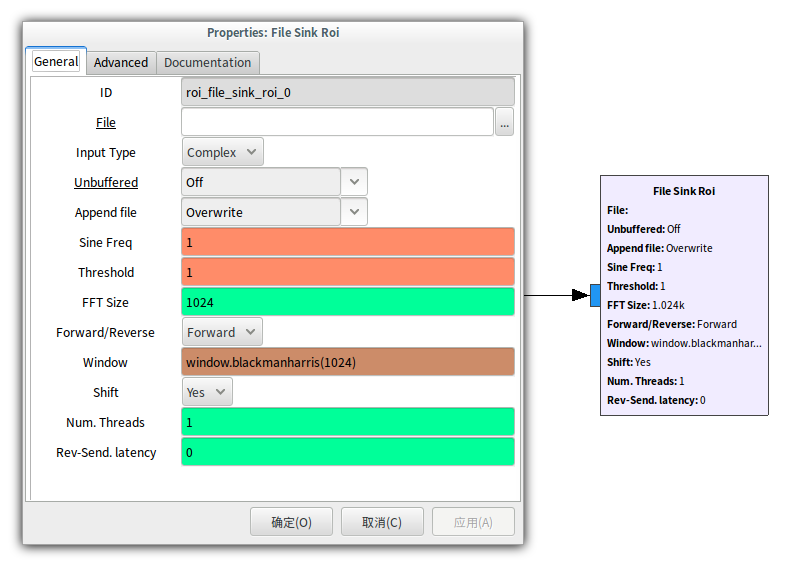
\includegraphics[width=0.9\textwidth]{images/file_sink_roi}
    \caption{导频信号检测模块}{} 
    \label{file_sink_roi}
\end{figure}

\subsection{导频信号收发机的整体结构}

本文基于上述四个GNURadio模块搭建导频信号收发机,整体结构如图\ref{two_tranceiver_structure2}所示。上层程序通过控制Alice的导频序列发射模块,发射导频信号,将导频信号调制到指定频点,并通过USRP射频前端发射导频信号。Bob使用导频信号检测模块不断检测导频信号,当检测到指定导频信号时,转存到磁盘,并触发导频信号发射事件,通知发射机中的导频序列发射模块发射导频信号,Bob端的发射机发射导频信号之后,Alice端接收机中的导频信号检测模块可以检测到Bob端发射的导频信号,并转存导频信号到磁盘。一次信道探测过程完成。

实际上,检测算法由于阈值设定过高或者过低,有可能检测不到对方发射的导频信号或者将错误的信号数据误认为导频信号。因此Alice端设计了重发机制。在一次信道探测过程中,Alice会每隔一定时间,重新发射一次导频信号,直到检测到Bob回发的导频信号。

\begin{figure}
    \centering
    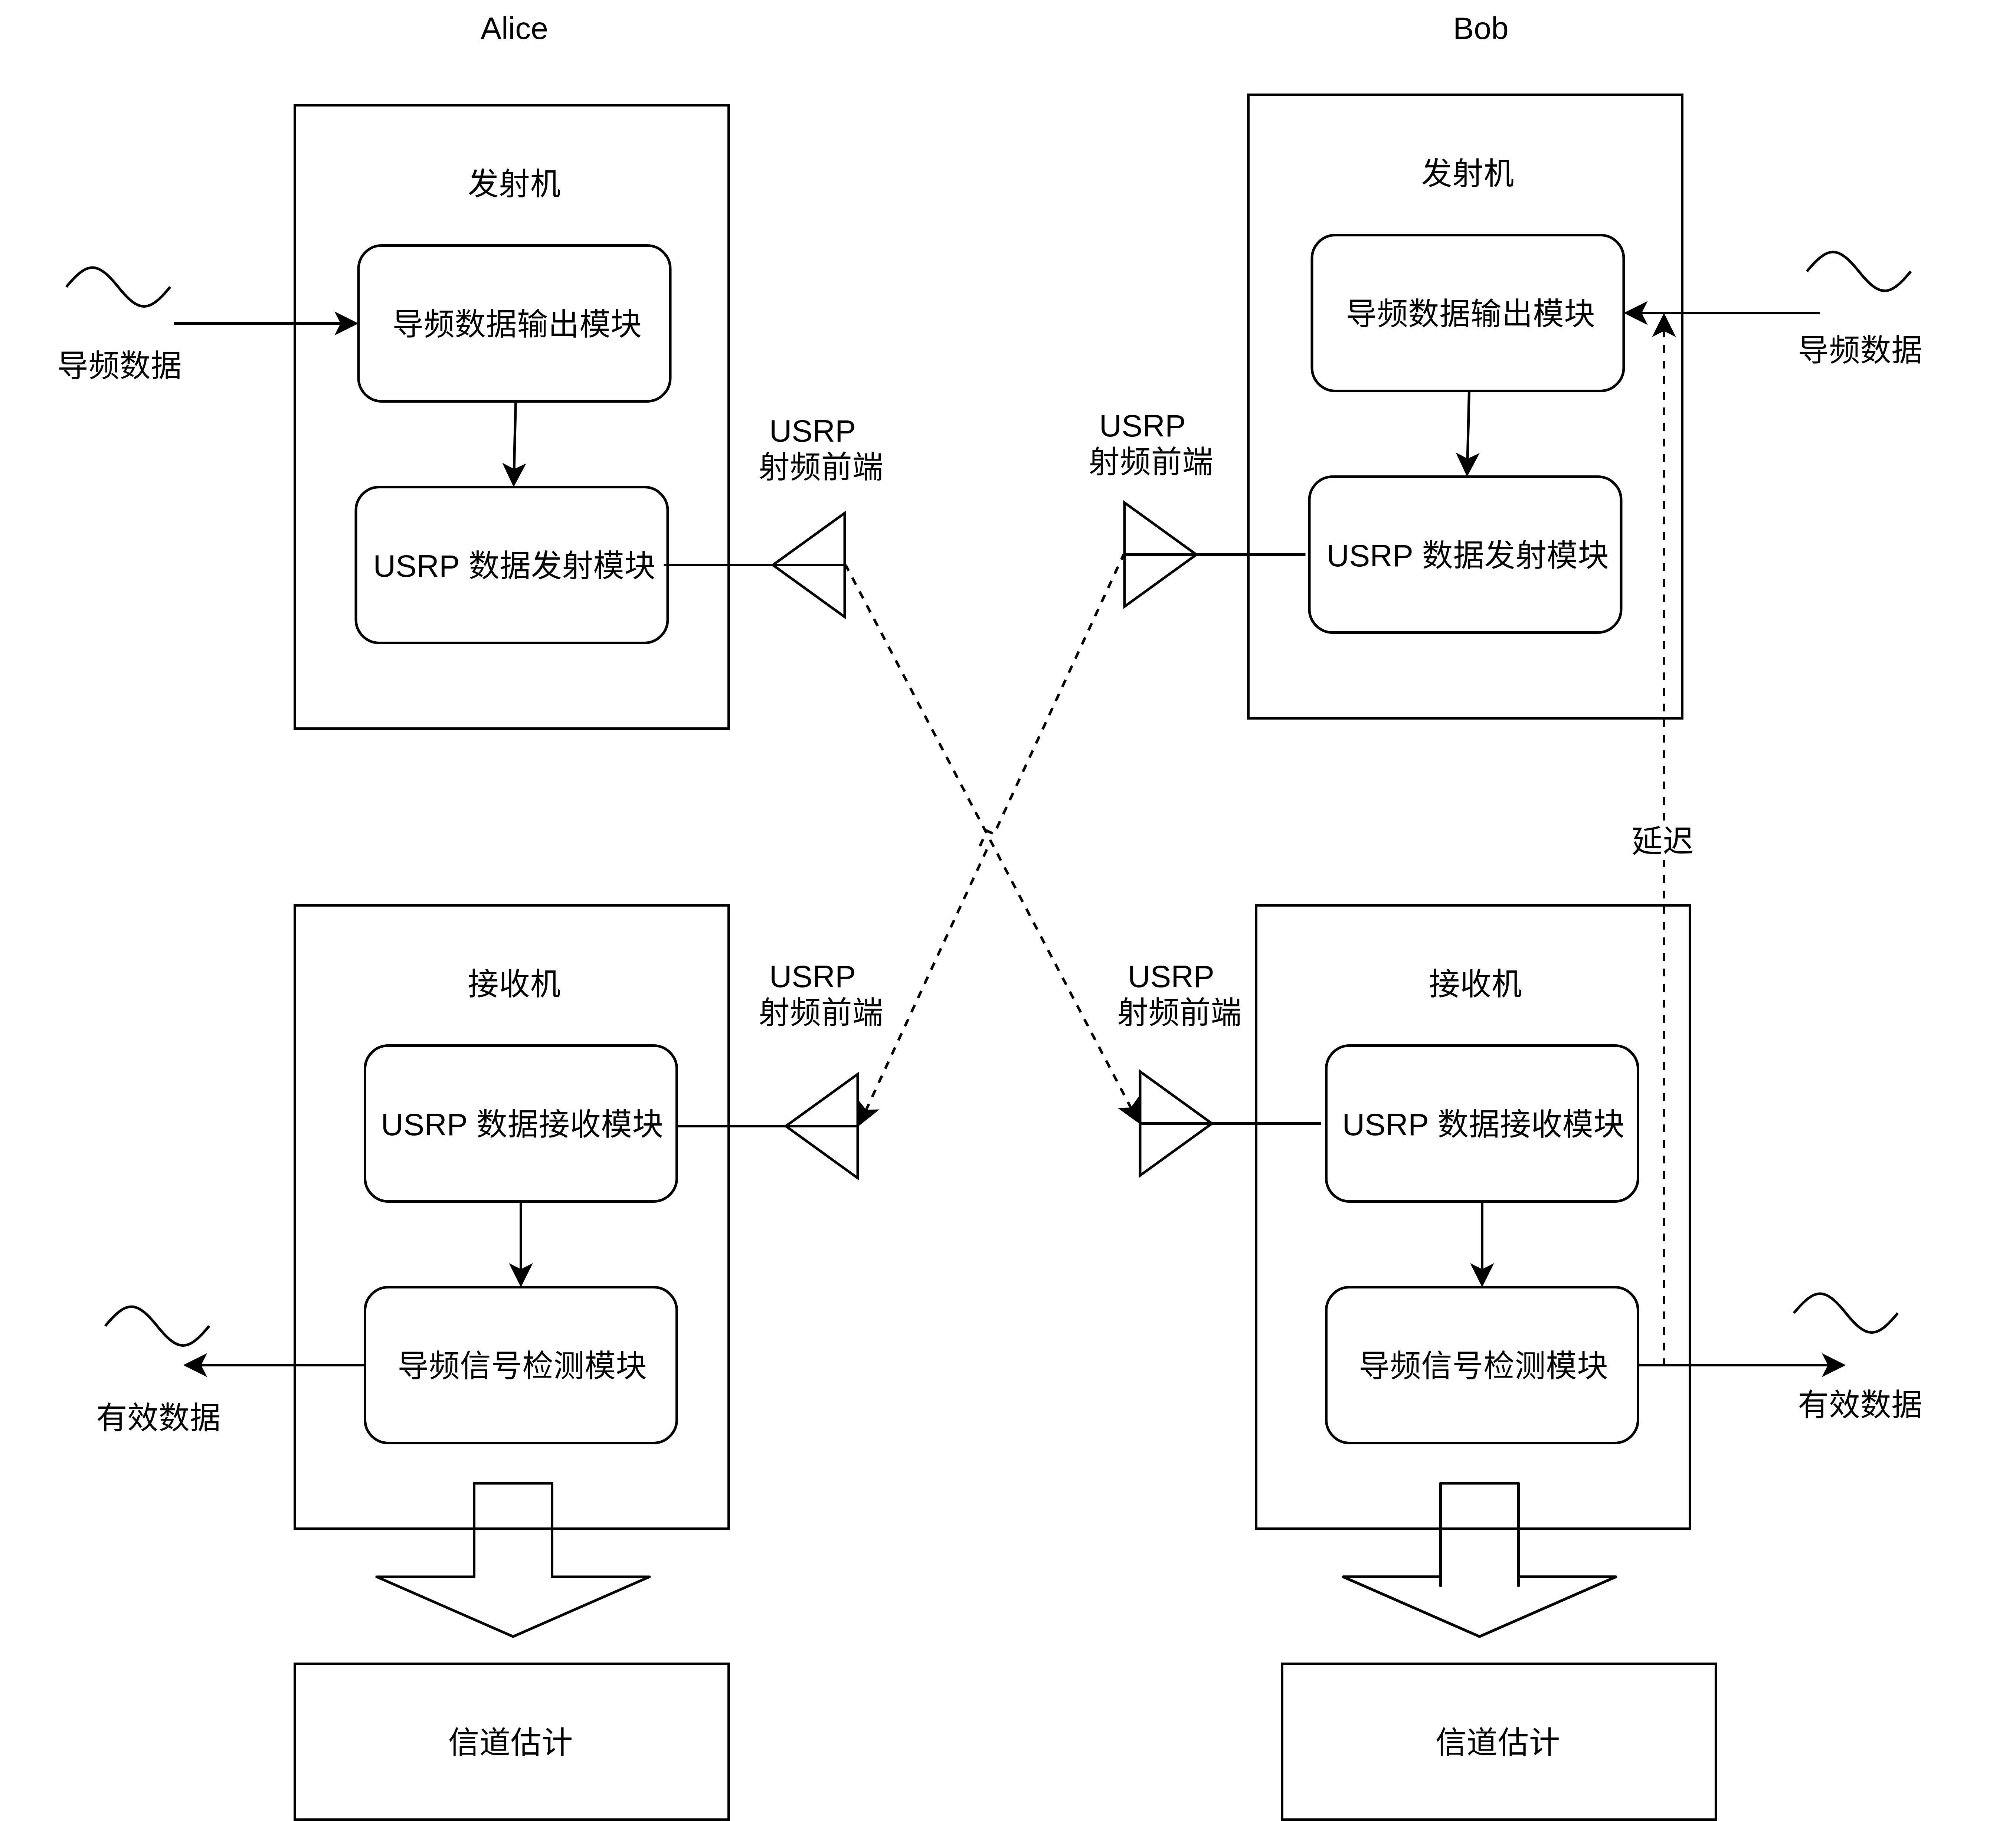
\includegraphics[width=0.9\textwidth]{images/two_tranceiver_structure2}
    \caption{TDD导频收发机设计}{} 
    \label{two_tranceiver_structure2}
\end{figure}

\chapter{无线信道密钥生成流程}

本章将详细的介绍无线密钥生成系统设计和实现的具体细节,介绍上层应用利用导频信号收发机实现信道探测的过程。% TODO 补完介绍

\section{TDD/FDD系统信道探测系统研究设计}

在上一章节中,本文介绍了如何利用GNURadio设计密钥生成系统所需要的模块搭建导频信号收发机,导频信号收发机使用如图\ref{tranceiver_structure}四个模块完成TDD/FDD系统中信号的发送和接收。

\begin{figure}
    \centering
    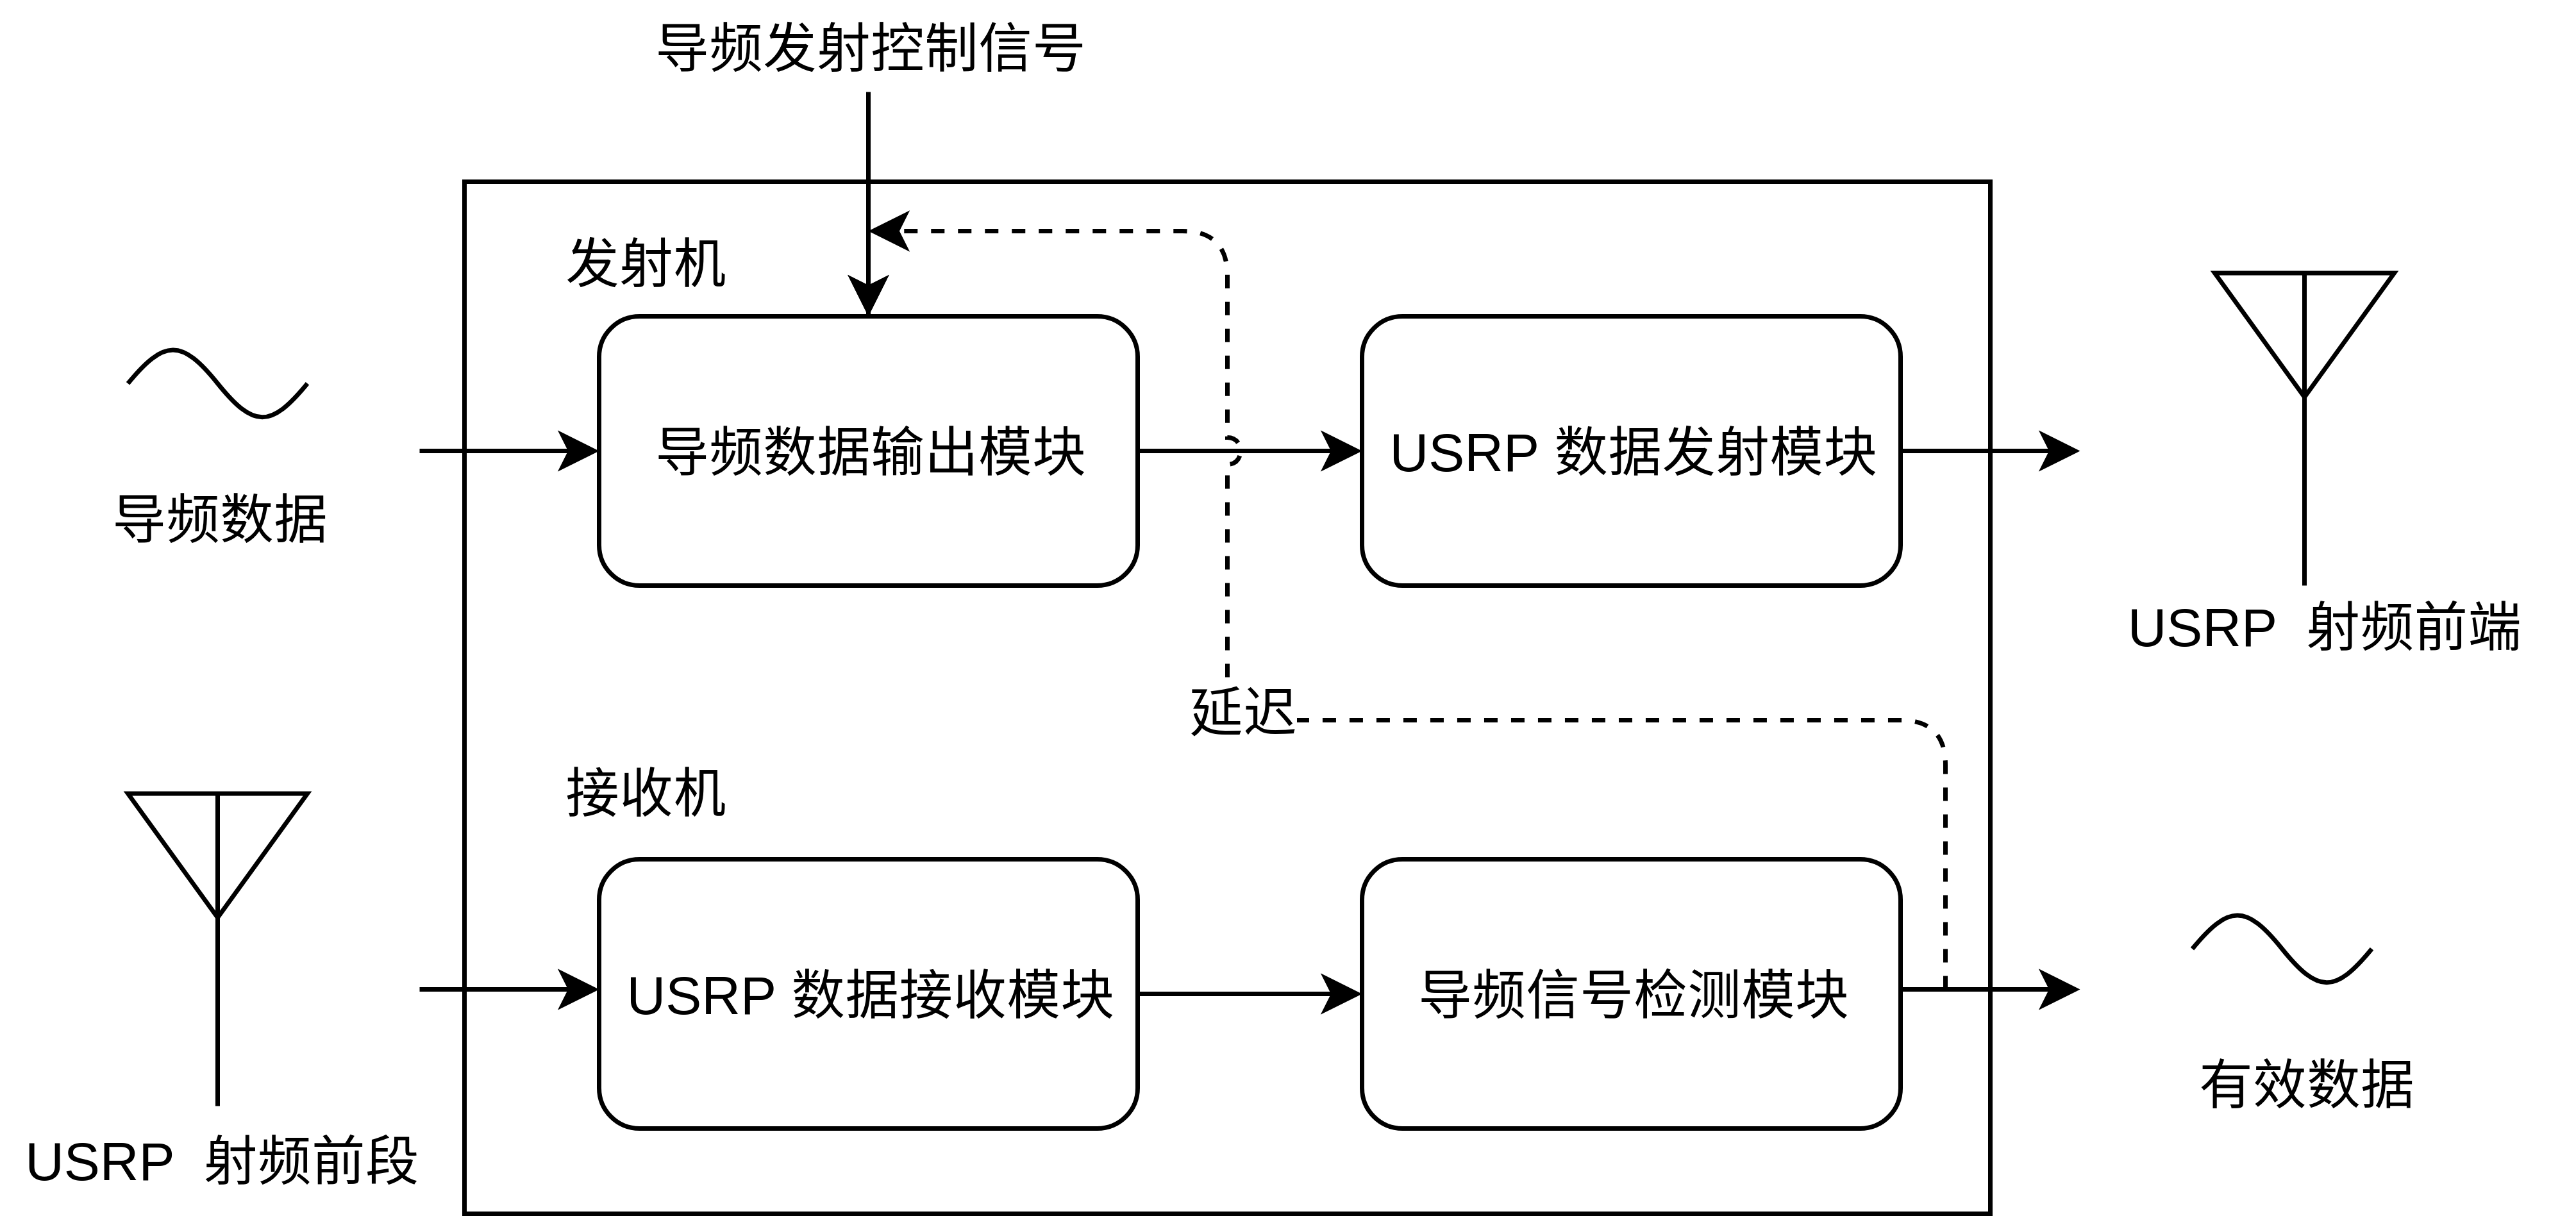
\includegraphics[width=0.9\textwidth]{images/tranceiver_structure}
    \caption{导频信号收发机}{} 
    \label{tranceiver_structure}
\end{figure}

对于TDD系统来说,Alice与Bob之间的信道探测过程如图\ref{two_tranceiver_structure}所示。对于FDD系统来说,Alice与Bob之间的信道探测过程如图\ref{two_tranceiver_structure2}所示。TDD和FDD系统中不同的地方在于,TDD系统的通信双方在同一个频点上发射和接收导频信号,而FDD系统的通信双方在不同的频点上发射和接收导频信号。


\begin{figure}
    \centering
    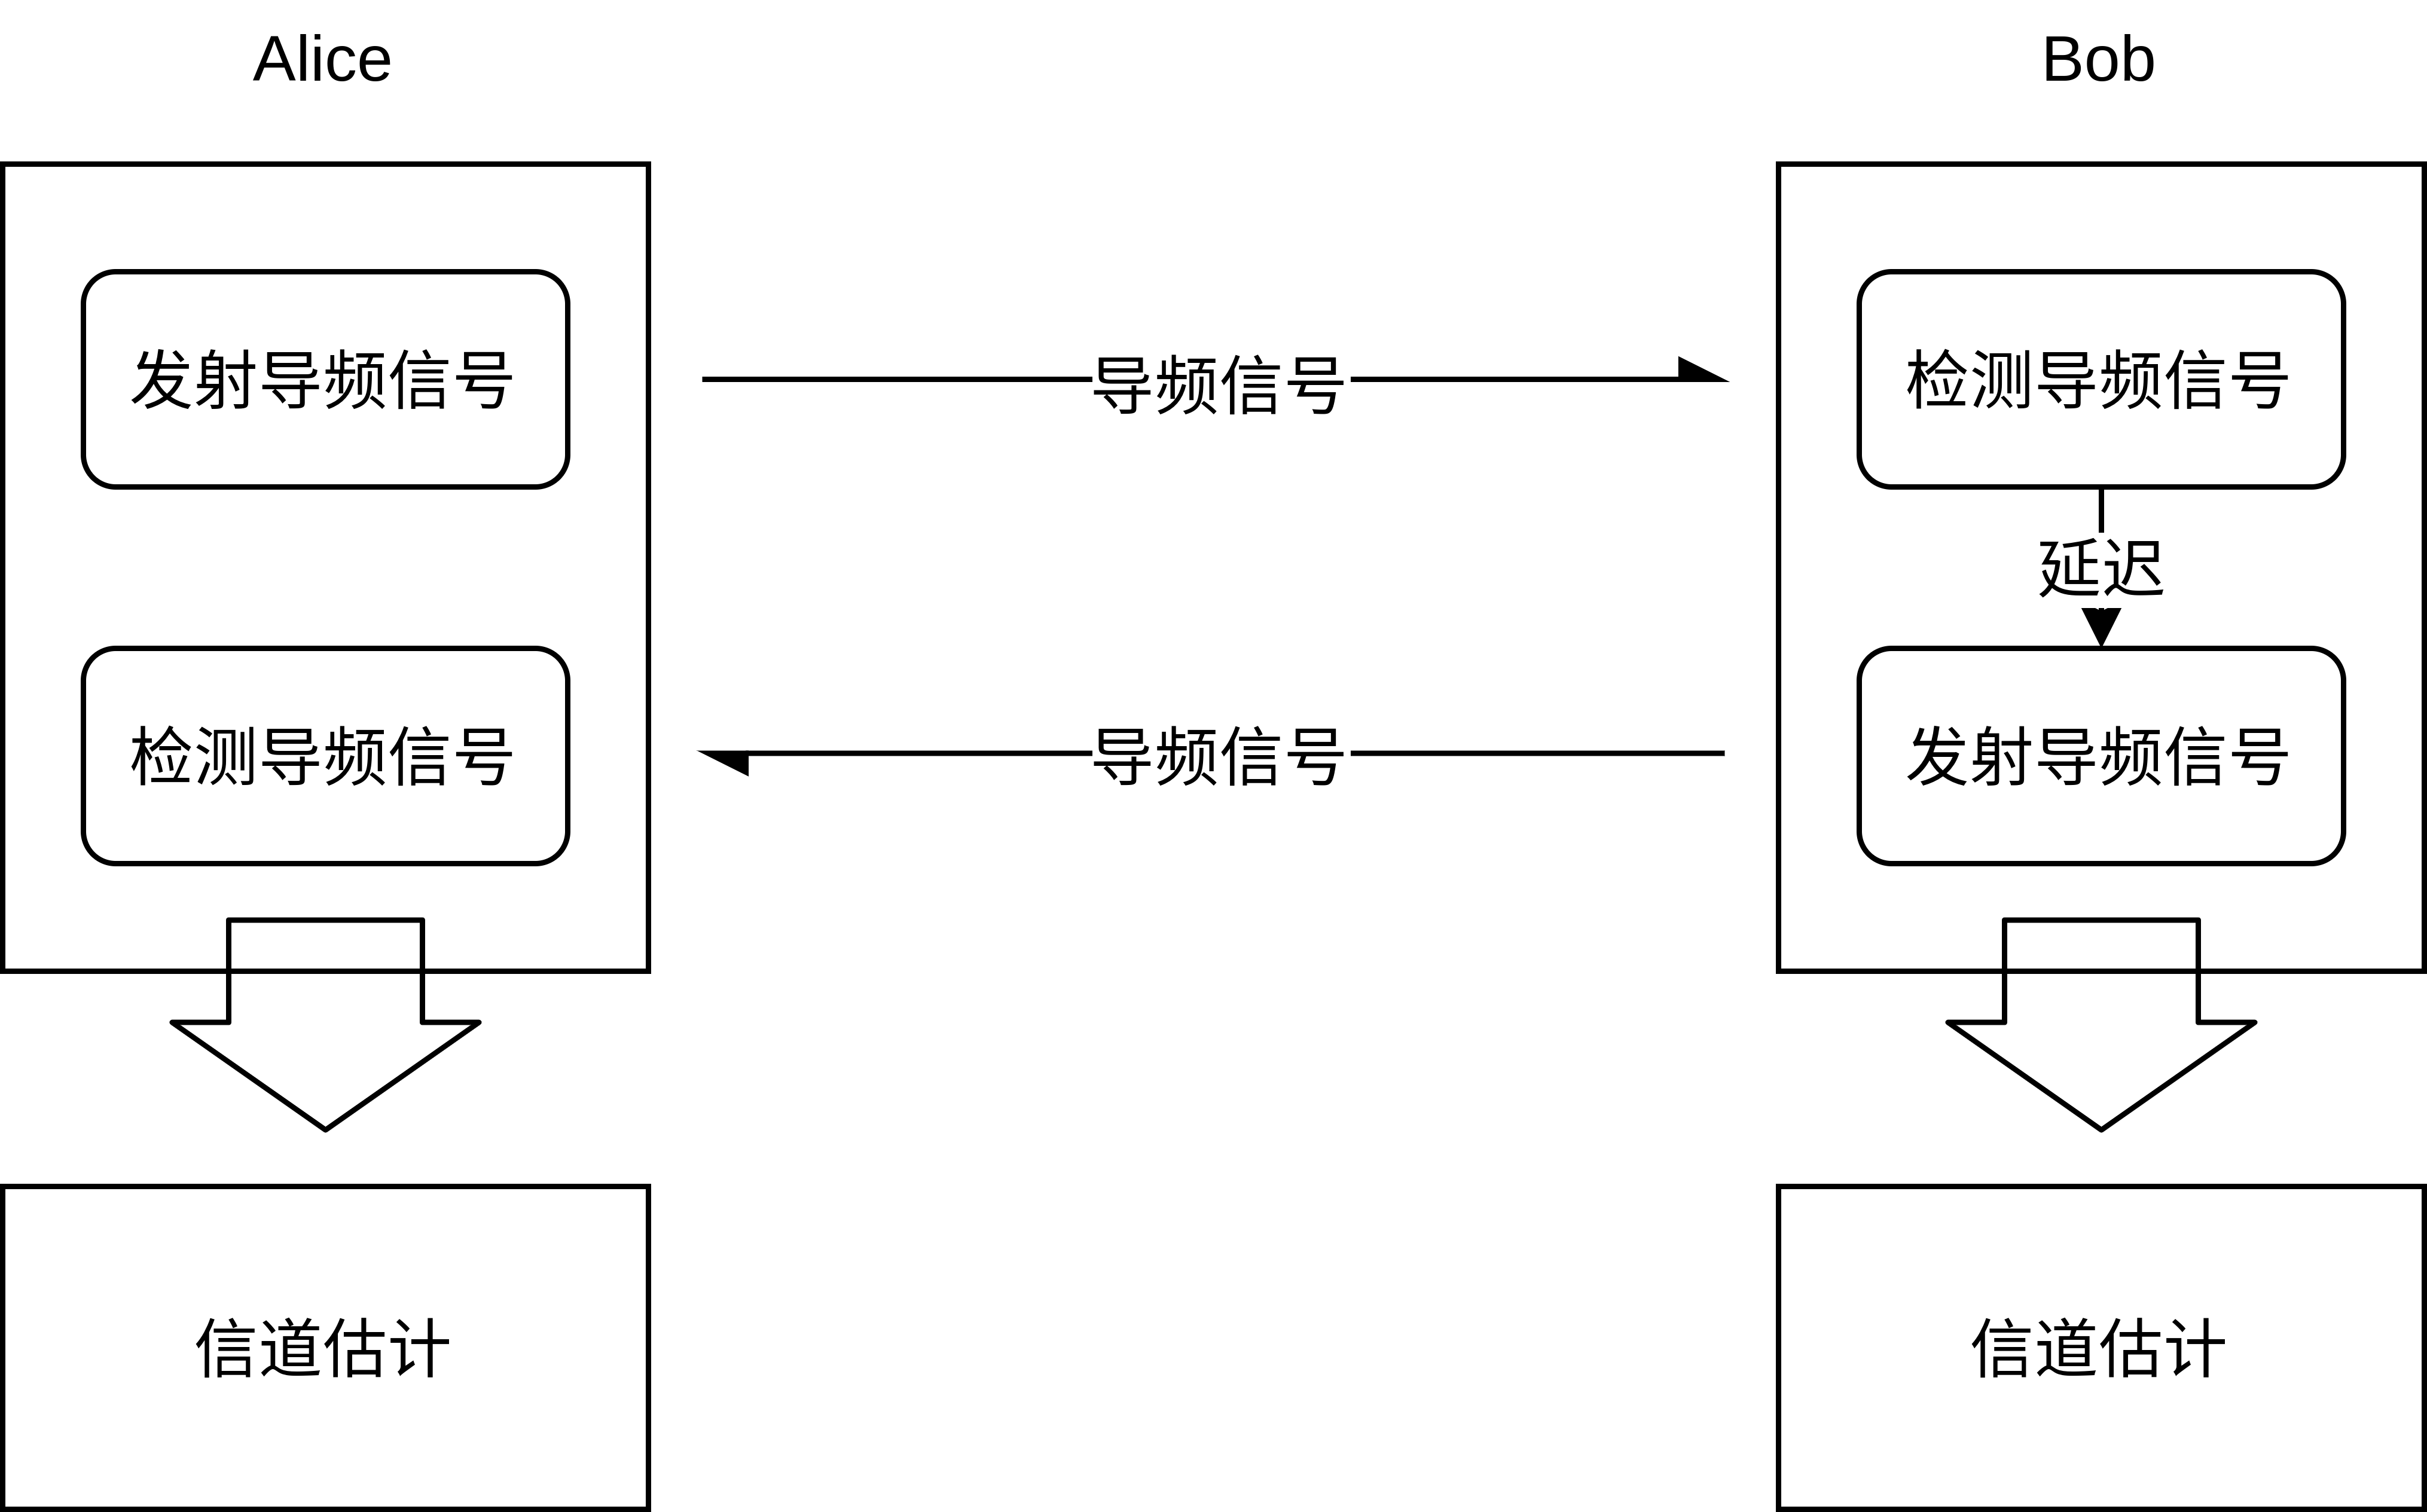
\includegraphics[width=0.9\textwidth]{images/two_tranceiver_structure}
    \caption{TDD系统中的信道探测}{} 
    \label{two_tranceiver_structure}
\end{figure}

\begin{figure}
    \centering
    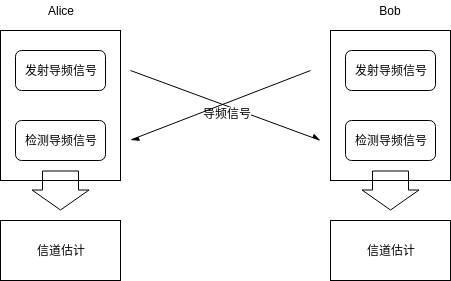
\includegraphics[width=0.9\textwidth]{images/two_tranceiver_structure_fdd}
    \caption{FDD系统中的信道探测}{} 
    \label{two_tranceiver_structure_fdd}
\end{figure}

TDD系统中,通信双方分Master和Slave端。Slave端的检波模块只有检测到Master端发射的导频信号,才会发射导频信号,因此Slave端的导频信号检测模块和导频序列输出模块之间存在信号事件。FDD系统中,通信双方的地位是对等的,不分主从,Slave发射导频信号是不受Master影响的,因此导频信号检测模块和导频序列输出模块之间也不存在信号事件。

为了实现信号事件,本文使用GNURadio中$gr::basic_block$提供的消息传递接口。在GNURadio中,$gr::basic_block$是所有模块的父类,模块也会区分输入和输出端口。该类提供了消息订阅与通知机制,如果某个模块注册了某个端口,那么当该模块在该端口发布消息时,任何订阅该模块同名端口的模块都会收到该消息并根据消息类型作出不同的响应行为。实际上,当模块在某端口发布消息时,该模块会迭代所有订阅同名端口的模块,并调用成员方法将消息压入到订阅模块的消息队列中去,如图\ref{message_passing}所示。本文实现了导频信号检测模块和导频序列输出模块之间的消息通知,并加入延迟这一参数观察不同延迟时间下信道和密钥生成的结果。

\begin{figure}
    \centering
    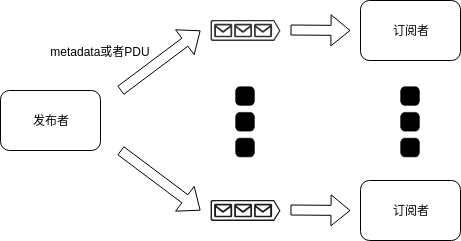
\includegraphics[width=0.9\textwidth]{images/message_passing}
    \caption{消息传递接口}{} 
    \label{message_passing}
\end{figure}

\section{信道估计}

本文使用的导频信号如图\ref{}所示,系统检波得到的导频信号如图\ref{}所示。在密钥生成协议中,通信双方均已得知导频信号的组成部分,因此可以通过已知导频信号和接收导频信号估计得到信道。

\section{特征量化}
\section{信息调和}
\section{隐私放大}

\chapter{实验和数据}

\section{场景架构与分析}
\section{实证分析}
\section{实证小结}

\chapter{总结展望}

\end{Main} % 结束正文

\begin{Acknowledgement}{}
这次的毕业论文设计总结是在我的指导老师xxx老师亲切关怀和悉心指导下完成的。从毕业设计选题到设计完成,x老师给予了我耐心指导与细心关怀,有了莫老师耐心指导与细心关怀我才不会在设计的过程中迷失方向,失去前进动力。x老师有严肃的科学态度,严谨的治学精神和精益求精的工作作风,这些都是我所需要学习的,感谢x老师给予了我这样一个学习机会,谢谢!

  感谢与我并肩作战的舍友与同学们,感谢关心我支持我的朋友们,感谢学校领导、老师们,感谢你们给予我的帮助与关怀;感谢肇庆学院,特别感谢计算机科学与软件学院四年来为我提供的良好学习环境,谢谢!
\end{Acknowledgement}

% 参考文献
\bibliography{seuthesis}



\newpage
\printindex % 索引

%\begin{thebibliography}{99}


% \bibliographystyle{ieee}
% \bibliography{seuthesis}


\end{document}
